\documentclass[12pt]{article}

\usepackage{notestyle}

\usepackage{bookmark}

\graphicspath{ {./img/} }


\title{Appunti Architettura}
\author{Brendon Mendicino}



\begin{document}

\maketitle
\newpage
\tableofcontents
\newpage


\section{Introduzione}\label{sec:introduzione}
Nell'introduzione si parla di roba, tipo evoluzione dei processori e del marcato intorno ad essi... Si parla della \textbf{legge di Amdahl} che calcola lo speedup di un processore con dei miglioramenti.
\[ \text{speedup} = \frac{\text{performance with enhancement}}{\text{performance without enhancement}} \]
Oppure:
\[ time_{new} = time_{old} \cdot \left( (1 - fraction_{enhanced}) + \frac{fraction_{enhanced}}{speedup_{enhanced}} \right) \]
\[ speedup_{overall} = \frac{time_{new}}{time_{old}}  = \frac{1}{\left( (1 - fraction_{enhanced}) + \frac{fraction_{enhanced}}{speedup_{enhanced}} \right)} \]
\begin{figure}[H]
    \centering
    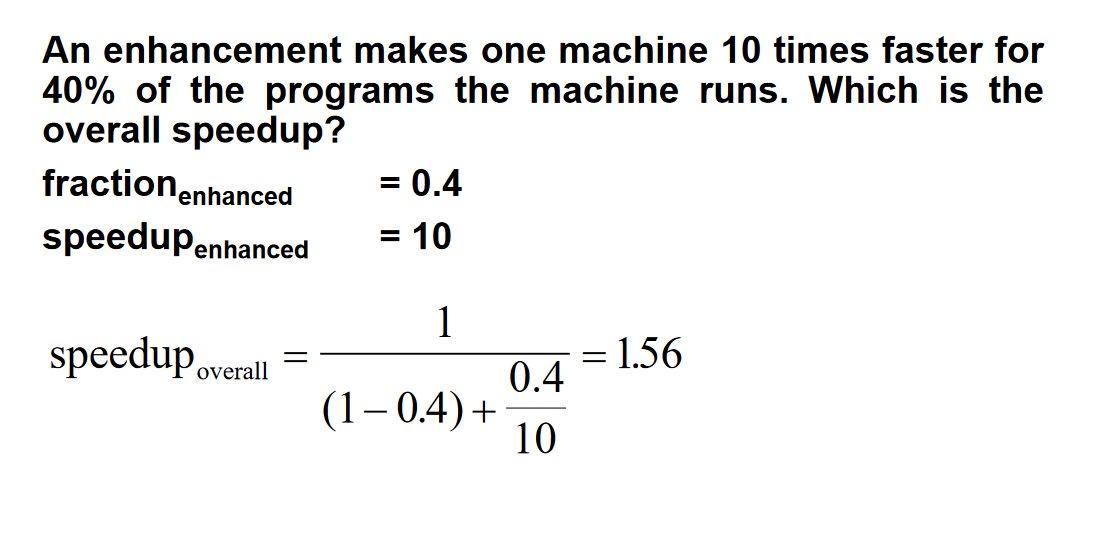
\includegraphics[width=0.8\textwidth]{amdahl-example.png}
    \caption{Amdahl Example}
    \label{fig:amdahl-example}
\end{figure}

\subsection{Addressing Mode}
Esistono modi di indirizzamento che si possono usare quando si progetta un ISA:
\begin{itemize}
    \item register mode: add r4, r3;
    \item immediate mode: add r4, \#4;
    \item displacement mode: add r4, 100(r3);
    \item register deferred mode: add r4, (r3);
    \item indexed mode: add r4, (r3 + r2);
    \item direct mode: add r4, (1001); 
    \item memory indirect mode: add r1, @(r3);
    \item autoincrement mode: add r1, (r3)+;
    \item autodecrement mode: add r1, -(r3);
    \item scaled mode: add r1, 100(r3)[r2];
\end{itemize}

\subsection{MIPS}
Tipi di istruzion nel mips sono:
\begin{itemize}
    \item immediate;
    \item register;
    \item jump;
\end{itemize}

\newpage
\section{Pipeline}
Per misurare le prestazioni di una pipeline si usa il \textbf{throughput}. Il throughput \`e il numero di sitruzioni che escono dalla pipeline in un intervallo di tempo.
\begin{figure}[H]
    \centering
    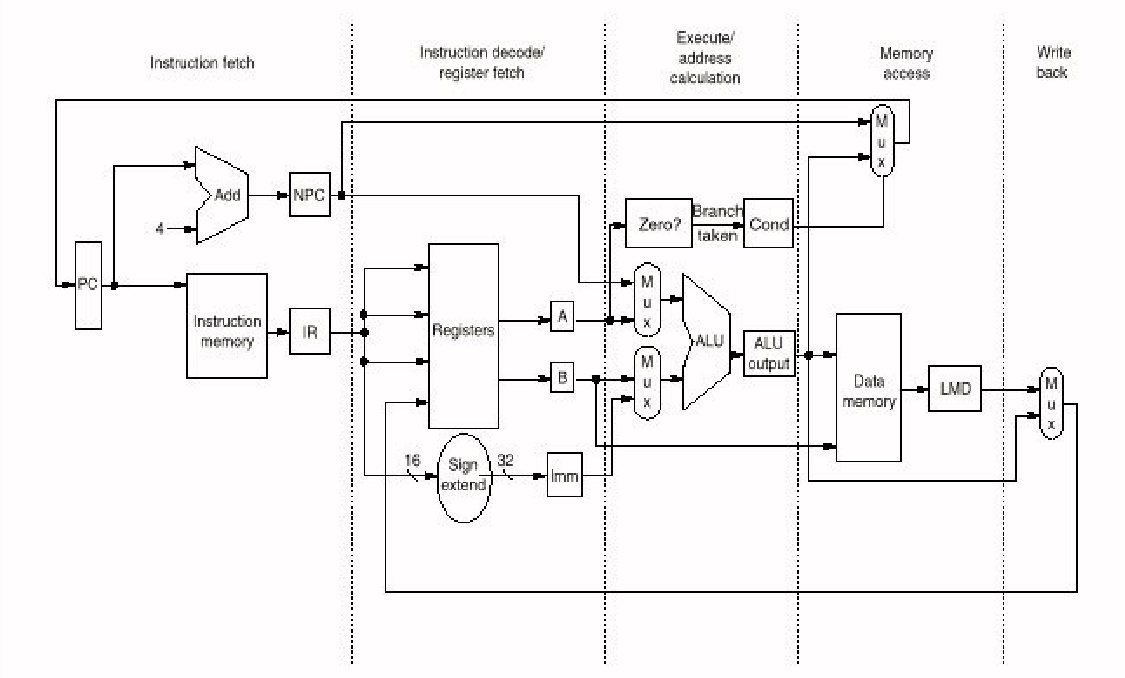
\includegraphics[width=0.8\textwidth]{datapath.png}
    \caption{Datapath}
    \label{fig:datapath}
\end{figure}
Il datapath \`e composto da:
\begin{itemize}
    \item instruction fetch: si prende dalla memoria la prossima istruzione putnatata dal PC e si incrementa quest'ultimo di 4;
    \item decode: si decodifica l'istruzione, attivando il datapath in modo adeguato, a prescindere dal tipo di operazione carico i due registri rs ed rt, ed il campo immediato, anche nel caso l'istruzione non fosse immediata, risparmio del tempo aumentando leggermente il comsumo di potenza;
    \begin{itemize}
        \item A $\leftarrow$ Reg[rs];
        \item B $\leftarrow$ Reg[rt];
        \item Imm $\leftarrow$ ($IR_{16\dots 31}$);
    \end{itemize}
    \item execution/effective address cycle: 
        \begin{itemize}
            \item memory reference: ALUoutput $\leftarrow$ A + Imm;
            \item register-register: ALUoutput $\leftarrow$ A op B;
            \item register-immediate: ALUoutput $\leftarrow$ A op Imm;
            \item brach: ALUoutput $\leftarrow$ NPC + Imm; Cond $\leftarrow$ (A op 0);
        \end{itemize}
    \item memory access/branch completion cycle:
        \begin{itemize}
            \item LMD $\leftarrow$ Mem[ALUoutput]; or Mem[ALUoutput] $\leftarrow$ B;
            \item branch: if (cond) PC $\leftarrow$ ALUoutput else PC $\leftarrow$ NPC;
        \end{itemize}
    \item write-back cycle:
        \begin{itemize}
            \item register-register: Reg[$IR_{16\dots 20}$] $\leftarrow$ ALUoutput;
            \item register-immediate: Reg[$IR_{11\dots 15}$] $\leftarrow$ ALUOutput;
            \item load instruction: Reg[$IR_{11\dots 15}$] $\leftarrow$ LMD;
        \end{itemize}
\end{itemize}

L'assunzione molto forte sar\`a che tutti i dati e le istruzioni saranno sempre nelle memoria cache, quindi si avr\`a un delay di un solo colpo di clock. Il register file potr\`a sia essere letto che scritto, ci sar\`a dunque bisogno di soddisfare queste richeste in un solo colpo di clock, la scrittura avviene nella prima parte del colpo di clock mentre la lettura avviene nelle seconda parte del colpo di clock.

Si aggiungono dei registri (detti pipeline register), 

Aggiungere i registri della pipeline aggiunge un overhead, inoltre il clock del processore comporta un rallentamento causato dallo skew, ma questo garantisce l'utilizzo istantaneo dei registri per la pipeline.

\subsection{Pipeline Hazards}
Sono dei casi in cui l'istruzione non pu\`o essere esguita in modo corretto nel suo slot temporale di esecuzione:
\begin{itemize}
    \item structural hazards: dipendono da conflitti su risorse;
    \item data hazards: dipende dal risultato di istruzioni precedenti;
    \item control hazards: dependi dai branch e da istuzioni che modificano il PC;
\end{itemize}

\paragraph{Stall}
Un modo di gestire gli hazards \`e di manadre la CPU in stallo.

\paragraph{Structural hazards}
Gli hazard strutturali possono essere:
\begin{itemize}
    \item un istruzione non riesce a completare un unit\`a in un solo colpo di clock (come l'unit\`a di divisione);
    \item la pipeline ha un accesso a memoria con un singola porta, e pi\`u istruzioni vorrebbero accedere contemporaneamente alla memoria;
\end{itemize}
Risolvere gli hazard strutturali comporta un costo, in termini di nuovo hardware e di migliorare quello esistente. Un processore con hazard strutturali avr\`a un clock pi\`u veloce ma problemi di accesso alla memoria, un processore senza hazard strutturali avr\`a un clock pi\`u lento ma nessuna limitizione di accesso alla memoria.

\paragraph{Data hazards}
Generati dalle dipendenze dei dati generati all'interno della pipeline. Esempio:
\begin{lstlisting}
add r1, r2, r3
sub r4, r1, r5
and r6, r1, r7
or  r8, r1, r9
xor r10, r1, r11
\end{lstlisting}
Il registro r1 viene inizializzato nella prima istruzione e poi utilizzato nel resto del codice, ma l'operazione di scrittura in si trova alla fine della pipeline, l'istruzione successiva (sub) dovrebbe aspettare che r1 sia scritto prima che possa essere letto, se tuttavia si tenta di leggere r1 il risultato sar\`a non deterministico. Per risolvere questo problema si hanno due soluzioni:
\begin{itemize}
    \item mandare in stallo il processore;
    \item implementiamo un forwarding che permette di non attendere la scrittura del registro, ma di leggere direttamente il valore dei registri della pipeline;
\end{itemize}
\begin{figure}[H]
    \centering
    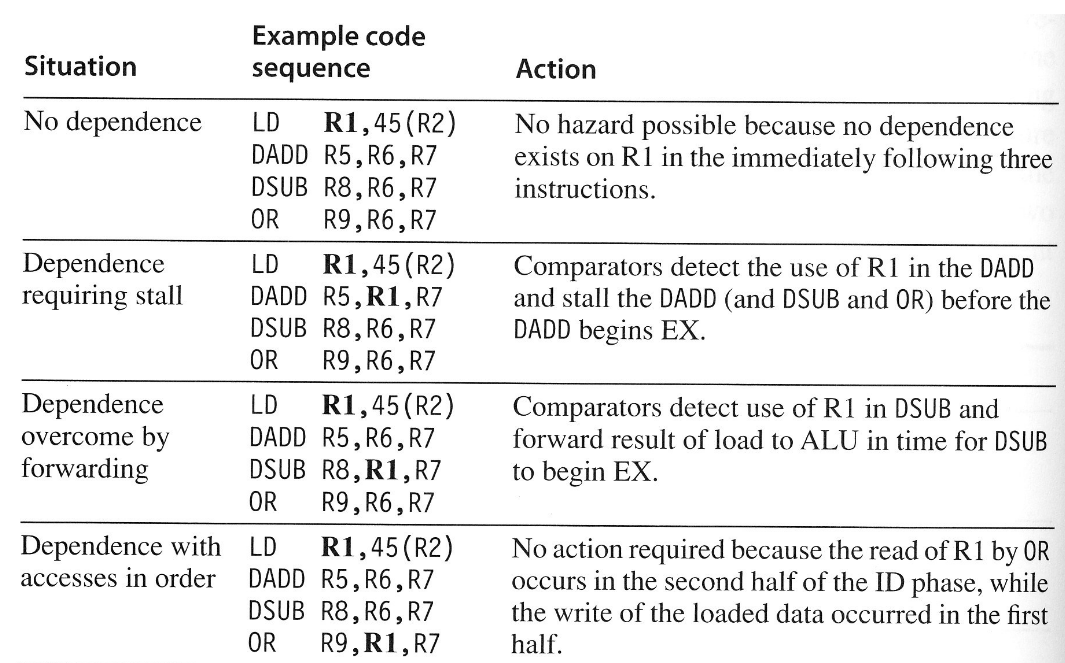
\includegraphics[width=0.8\textwidth]{load-interlock-detection.png}
    \caption{Load Interlock Detection}
    \label{fig:load-interlock-detection}
\end{figure}

\paragraph{Control Hazards}
I contrl hazard sono causati da istruzi di branch, il loro effetto in casa di salto positivo \`e quello si svuotare l'intera pipeline per porter rimuovere le istruzioni seccessive al branch e inseririre quelle del nuovo PC. I modi per migliorare gli effetti dei branch sono:
\begin{itemize}
    \item freezing the pipeline: stall o flush della pipeline;
    \item predict untaken: considera il branch come non preso;
    \item predict taken: consedera il branch come sempre preso;
    \item delayed branch;
\end{itemize}



\subsection{Floating Point}
Le operazioni floating point sono molto complesse, se si cerca di implementarle in un solo colpo di clock allora il processore diventa troppo complicato dal punto di vista logico, un altra soluzione potrebbe essere quello di rallentare il clock, per far entrare tutte le operazioni in un singolo colpo, ma entrambe le soluzioni non sono fattibili, allora si prende un approcia di suddivisione della pipeline in unit\`a. Per supportare le operazioni di floating point in pipeline, si \`e optato per una separazione dalla execute in diverse unit\`a:
\begin{itemize}
    \item integer unit;
    \item fp/integer multiply;
    \item fp adder;
    \item fp/integer divider;
\end{itemize}
Questa ramificazione della pipeline va a convergere nella sezione di MEM.

Si dovr\`a definire la latenza, ovvero il numero di colpi di clock che una unit\`a usa per avere un risultato, ed un intervallo di inizializzazione, ovvero il numero di colpi di clock che la seconda istruzione davr\`a attendere per entrare nella sezione desiderata (come somma o divisione). Un esempio:
\begin{itemize}
    \item add: lat: 1, int: 1;
    \item mult: lat: 8, int: 1;
    \item fadd: lat: 4: 1;
    \item div: lat: 24, int: 24;
\end{itemize}
\begin{figure}[H]
    \centering
    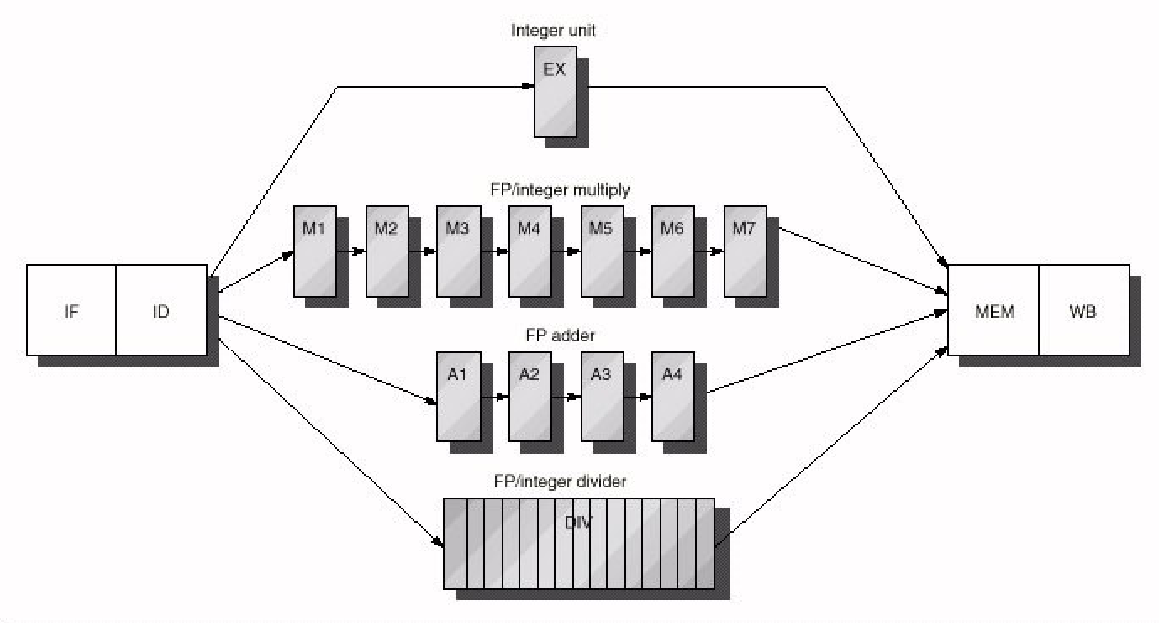
\includegraphics[width=0.8\textwidth]{pipeline-units.png}
    \caption{Pipeline Units}
    \label{fig:pipeline-units}
\end{figure}

Solitamente la divisione ha la latenza identica all'intervallo di inizializzazione. Se un unit\`a \`e \textbf{pipelined} allora ha un colpo di clock come intervallo di inizializzazione, se l'unit\`a non \`e pipelined allora il suo intervallo di inizializzazione \`e uguale alla latenza.


Un altro porblema dato dagli hazard strutturali \`e il fatto che: pi\`u istruzioni non possono accedere in contemporanea alla fase di MEM o di WB, solitamente il criterio \`e FIFO, oppure si potrebbe dare maggiore priorit\`a alla istruzioni con il maggiore numero di clock.

Adesso che le istruzioni non hanno pi\`u il WB in ordine, si creare un nuovo tipo di data hazard detto \textbf{write after write} e \textbf{read after write}.
\begin{figure}[H]
    \centering
    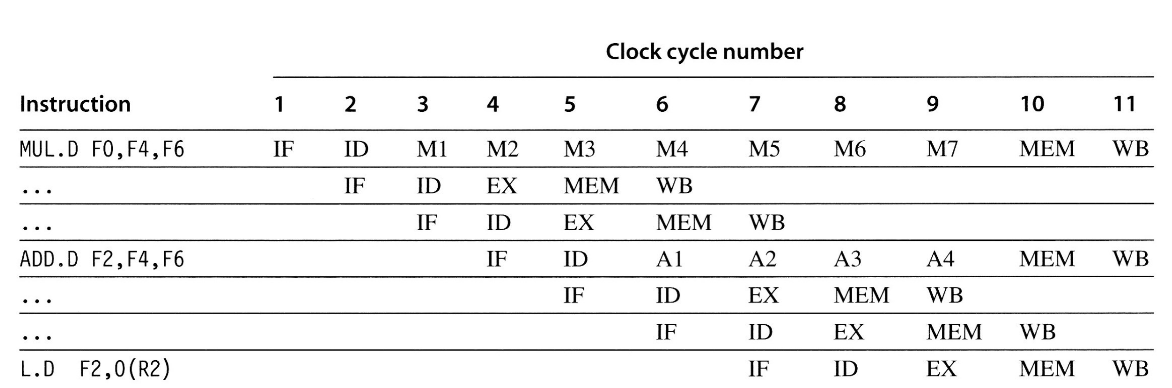
\includegraphics[width=0.8\textwidth]{write-after-wirte.png}
    \caption{Write After Wirte}
    \label{fig:write-after-wirte}
\end{figure}
In questo caso l.d e add.d scrivono nello stesso momento sul registro f2, essendo che add.d si trova prima della l.d l'operazione non pu\`o essere eseguita, una soluzione \`e: prima di schedulare un istruzione al EX stage, si deve controllare che non si stia scrivendo su un registro gi\`a presente nelle istruzioni in EX, se \`e vero si stalla l'istruzione corrente in ID.



\subsection{Exceptions}
Le eccezioni sono classificate in:
\begin{itemize}
    \tolerance=1000
    \item \textbf{sincrone} e \textbf{asincrone};
    \item \textbf{user requested} (l'utente potrebbe creare un eccezione) o \textbf{coerced} (data da fattori esterni);
    \item \textbf{maskable} o \textbf{non-maskable}: alcune eccezioni non sono mascherabili ovvero forzare l'hardaware a non rispondere all'exception;
    \item \textbf{within instructions} o \textbf{between instructions}: within all'interno delle istruzioni (metre un istruzione fa IF, ID, ...) oppure tra due istruzioni (ld, add);
\end{itemize}
Le macchine moderne sono chiamate \textbf{restartable machines} ovvero fanno ripartire il processore dallo stato in cui si trovava prima dell'eccezione. Quando una exception arriva al processore deve stoppare l'IF, fermare la scrittura della pipeline e riuscire a tornare dalla procedura da dove \`e stata chiamata l'exception.

\begin{example}{Interrupt protocal in 80x86}{interrupt-protocal-in-80x86}
    Quando la CPU rileva un interrupt, legge il tipo di interrupt dal bus, salva lo stato del processore
\end{example}

\begin{example}{Interrutp protocol in ARM}{interrutp-protocol-in-arm}
    Lla CPU salva lo Status Register, il PC ed il ed altri registri nello stack, aggiorna i flag, link register e PC  e salta al valore dell'exception.
\end{example}
Le eccezioni possono essere gestite in modo \textbf{preciso} o in modo \textbf{impreciso}:
\begin{itemize}
    \tolerance=1000
    \item preciso: quando arriva un interruzione, tutte le istruzioni che si trovano all'interno della pipeline devono essere completate e tutte quelle dopo devono essere rimandate, gestire questo tipo di istruzioni \`e molto oneroso;
    \item impreciso: un esempio eccezioni imprecise:
\begin{lstlisting}[language=]
div.d f0, f1, f2
sub.d f12, f12, f13
\end{lstlisting}
    se sub.d causa un eccezione allora viene detta imprecisa, perch\'e un istruzione precedente (div.d) si trova ancora nella pipeline. Per risolvere questo problema ci sono diverse scelte:
    \begin{itemize}
        \item forzare l'unit\`a di FP a non schedulare nuove istruzioni se pensa che una corrente possa causare un eccezione;
        \item bufferizzare il risultato finch\'e tutte le istruzioni precedenti non siano terminate;
        \item implementare una soluzione precisa solo per una unit\`a (tipo FP);
    \end{itemize}
\end{itemize}
Nel MIPS le possibili exception sono:
\begin{itemize}
    \item IF: page fault, accesso a memoria protetta;
    \item ID: opcode illegale;
    \item EX: exception aritmetiche;
    \item MEM: stesse della IF;
    \item WB: nussuna;
\end{itemize}
Se due exception arrivano nello stesso momento si po\`u creare un flag di status associato ad ogni istruzione, guardando se l'istruzione pu\`o causare un eccezione o meno, quando l'istruzione termina l'exception viene scatenata, cos\`i si crea un coda evitando exception simultanee, infatti ogni exception pu\`o essere scatenata solo al termine di ogni istruzione.


\subsection{Instruction Level Parallelism}
I processori cercano di sfruttare al massimo l'ILP, ovvero cercare di rischedulare le istruzioni in modo da evitare hazard il pi\`u possibile. L'ILP pu\`o essere:
\begin{itemize}
    \item \textbf{dinamico}: gestito dall'hrdware;
    \item \textbf{statico}: gestito a livello software, ovvero dal compilatore;
\end{itemize}
Solitamente questi due approcci possono essere combinati.

Il primo tipo di ILP \`e il \textbf{basic block}, dove si sceglie un blocco di istruzioni e si cerca di rischedularle per cercare di elimare gli hazard rispettando le dipendenze, questo blocco deve soddisfare due condizioni:
\begin{itemize}
    \item nessun branch pu\`o entrare nel blocco;
    \item nessum branch pu\`o uscire dal blocco;
\end{itemize}
Il motivo \`e che se queste due condizioni fossero possibili il codice perderebbe consistenza.

Un altro modo di aumentare il parallelismo \`e il \textbf{loop-level parallelism}, si cerca di fare un unrolling di un for loop (quando possibile), questo viene fatto per ridurre l'overhead causato dalle istruzioni di controllo.
\begin{figure}[H]
    \centering
    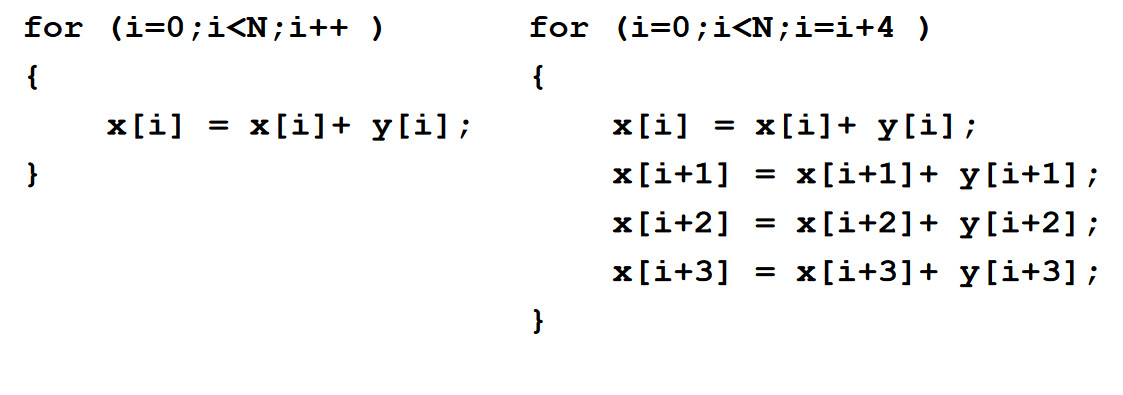
\includegraphics[width=0.8\textwidth]{loop-unrolling.png}
    \caption{Loop Unrolling}
    \label{fig:loop-unrolling}
\end{figure}
Il problema con questo approccio \`e che si aumenta la dimensione del codice.


\subsection{Dipendenze}
Esitono delle dipendende all'interno del codice, queste sono delle prorpriet\`a di come il codice \`e scritto, e non dalla pipeline come negli hazard.
\begin{enumerate}
    \item \textbf{Data Dependencies}: 
    \item \textbf{Memory Dependencies}:
    \item \textbf{Name Dependencies}:
\end{enumerate}

\subsection{Hazards}
Ogni volta che ci sono delle dipendenze tra i dati potrebbero presentarsi degli hazard, che vengono classificati in:
\begin{itemize}
    \item \textbf{RAW (read after write)}
    \item \textbf{WAW (write after write)}
    \item \textbf{WAR (write after read)}
\end{itemize}







\newpage
\section{Chache Memories}
\tolerance=1000
Le cache volocizzano l'accesso al memoria secondaria che \`e il collo di bottiglia dell'intero sistema. Si \`e creata un gerarchia di memorie molto pi\`u veloci quanto pi\`u vicine si trovano al processore.
\begin{itemize}
    \item \textbf{reigistri}: 500 bytes, 500ps;
    \item \textbf{L1}: 64 KB, 2ns;
    \item \textbf{L2}: 256 KB, 10-20ns;
    \item \textbf{Memoria primaria}: 512 MB, 50-100ns;
    \item \textbf{Memoria secondaria flash}: 8 GB, 50$\mu$s;
\end{itemize}
La cache funzionano grazie ai principi di localit\`a:
\begin{itemize}
    \item \textbf{temporale}: in un tempo $t_0 + \Delta t$ dal momento in cui ho letto un elemento, \`e probabile che il dato venga o l'istruzioe venga riusato;
    \item \textbf{spaziale}: in un spazio $x + \Delta x$ vicino all'elemento letto, \`e probabile che gli elementi vicini vengano letti;
\end{itemize}

\begin{theorem}{Cache Performance}{cache-performance}
    \begin{itemize}
        \item h: cache ratio;
        \item C: cache access time;
        \item M: memory access time;
    \end{itemize}
    Media del tempo di accesso:
    \[ t_{ave} = h * C + (1-h) * M \]
    Valori soliti per $h$ sono $0.9$.
\end{theorem}

\subsection{Organizzazione della cache}
Solitamente la cache \`e formata da una \textbf{parte di controllo} contenente il \textbf{cache controller} che controlla se accedendo alla cache \`e stato fatto un hit o un miss e in caso recupera la porzione di memoria, ed una \textbf{parte di dati} che contiene le \textbf{cache line} fatte da:
\begin{itemize}
    \item \textbf{validity bit}: il bit ci dice se la riga \`e valida o meno;
    \item \textbf{tag}: identifica il blocco di memoria presente nella riga;
    \item \textbf{data array}: contiene i dati presi dalla memoria;
\end{itemize}
A partire dall'indirizzo la cache si calcola un nuovo indirizzo di accesso alle righe, foramto da:
\begin{itemize}
    \item \textbf{tag}: identifica il blocco di memoria (bit dell'indirizzo - bit index - bit offset);
    \item \textbf{index}: riga della cache;
    \item \textbf{offset}: byte offset all'interno della riga;
\end{itemize}
Per regolare l'accesso alla cache il controllore identifica la riga attraverso l'index e comparando i due tag decide se \`e un hit o un miss, se \`e un hit ed il validity bit \`e a 1, allora attraverso l'offset viene prelevato il dato.

La cache si trovano tra il bus ed il processore, per evitare conflitti di utilizzo con perfiriferiche esterne o DMA.

Le cache moderne pi\`u vicine al processore sono separtate in \textbf{Instruction-Cache} e \textbf{Data-cache} (detta architettura di Harward), per evitare la lettura contemporanea di istruzioni e dati (structural hazard).

\subsection{Mappatura}
I tipi di mappatura (\textbf{associativity models}) sono:
\begin{itemize}
    \item \textbf{direct mapped}: la posizione nella riga \`e uguale a: \#block\_memory mod \#cache\_block;
    \item \textbf{set associative}: la cache viene partizionata in set di righe (i blocchi hanno tutti la stessa lunghezza, tipicamente 2 o 4), la posizione \`e determinata da: \#memory\_block mod \#sets, quando un altro blocco viene asseganto ad un set viene rimossa la riga meno utilizzata;
    \item \textbf{fully associative}: ogni blocco di memoria pu\`o essere salvata in qualsiasi riga della cache, questo ha come malus la perdita del campo index e l'indirizzo del blocco viene salvato per intero;
\end{itemize}

\paragraph{Algoritmi di rimpiazzamento}
Gli aloritmi usati per decidere quale riga rimpiazzare sono:
\begin{itemize}
    \item LRU (last recently used): il pi\`u usato;
    \item FIFO: il meno caro in termini di prestazioni;
    \item LFU (least frequently used): teorico, il pi\`u efficace;
    \item random: semplice ed efficace;
\end{itemize}

\subsection{Update della Memoria}
Quando un operazione di scrittura \`e fatta sulla cache deve anche essere propagata sulla memoria, le due possibili soluzioni a questo problema sono:
\begin{itemize}
    \item \textbf{write back}: per ongi riga della cache \`e introdotto un flag detto \textbf{dirty bit}, che indica quando i dati all'interno sono cambiati;
    \item \textbf{write through}: ogni volta che la CPU effettua un operazione di scrittura, i dati vengono scritti sia in cache sia in memoria, questa \`e la soluzione pi\`u usata per due motivi:
        \begin{itemize}
            \item le operazioni di scrittura sono meno frequenti di quelle di lettura, quindi ci si pu\`o permettere un po di overhead;
            \item in questo modo si risolvono tutti i problemi relativi alla gestione di scrittura in concorrenza, senza implementare altro hardware per la gestione di tale problematica;
        \end{itemize}
\end{itemize}





\newpage
\section{Branch Prediction}
Per effettuare delle predizioni esistono due tipi di approcci: prediction statici e prediction dinamici. Un esempio prediction statico \`e prendere tutti i salti come presi, oppure facciamo un filtro su quali tipi di branch prendere come presi (prendere i salti all'indietro come sempre presi). Per avere delle predizioni pi\`u accurate \`e usare un brach prediction dinamico (speculazione).

\subsection{Branch History Table}
Il BHT ha una memoria in cui sono contenute le informazioni relative ai salti. Si accede a questa tabella quando nella fase di fetch si prende un salto, si guarda l'informazione relativa al salto e si legge la predizione del salto.
\begin{figure}[H]
    \centering
    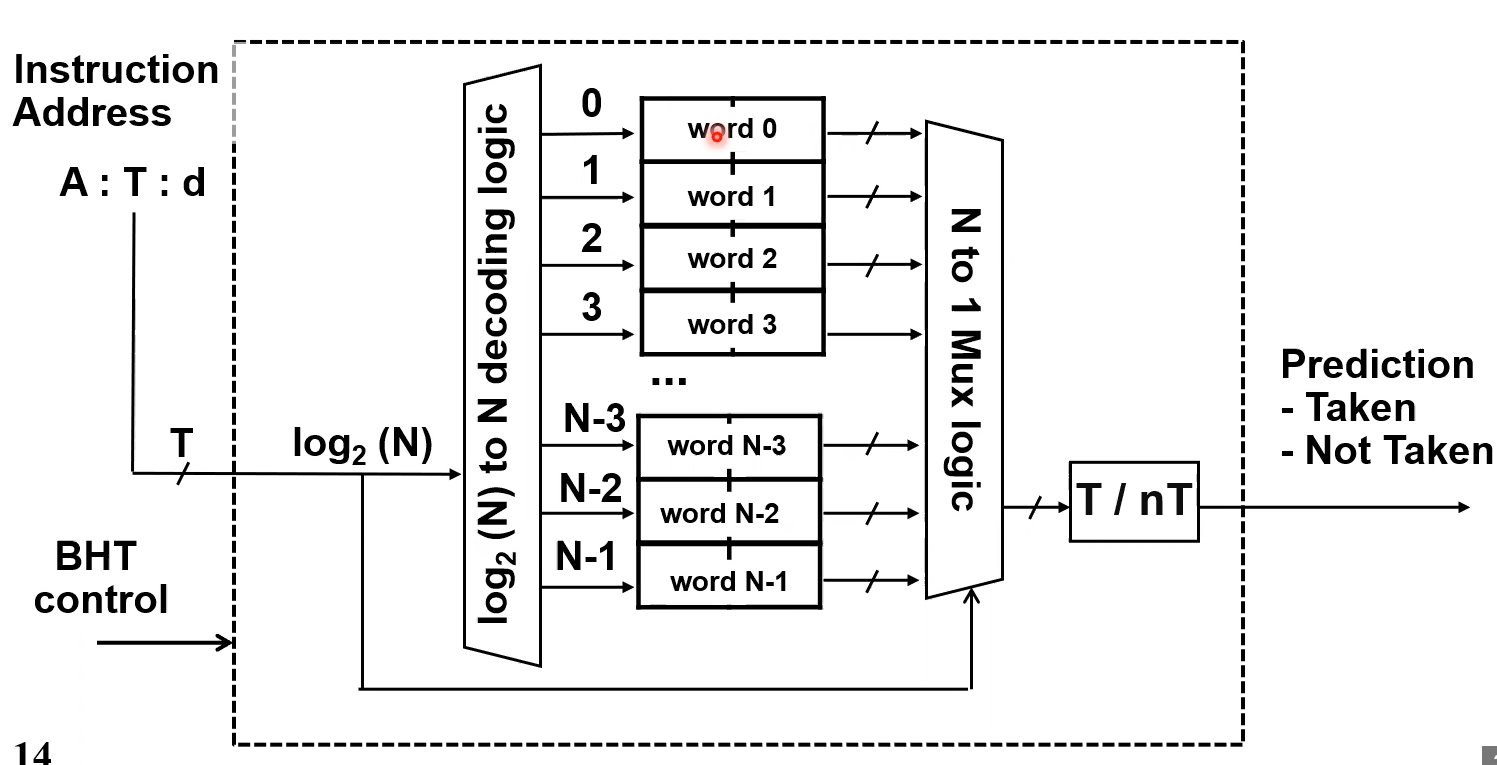
\includegraphics[width=0.8\textwidth]{bht-implementation.png}
    \caption{Bht Implementation}
    \label{fig:bht-implementation}
\end{figure}
Solitamente il valore che indica se il branch deve essere preso o meno solitamente \`e reppresentato da due bit.
\begin{figure}[H]
    \centering
    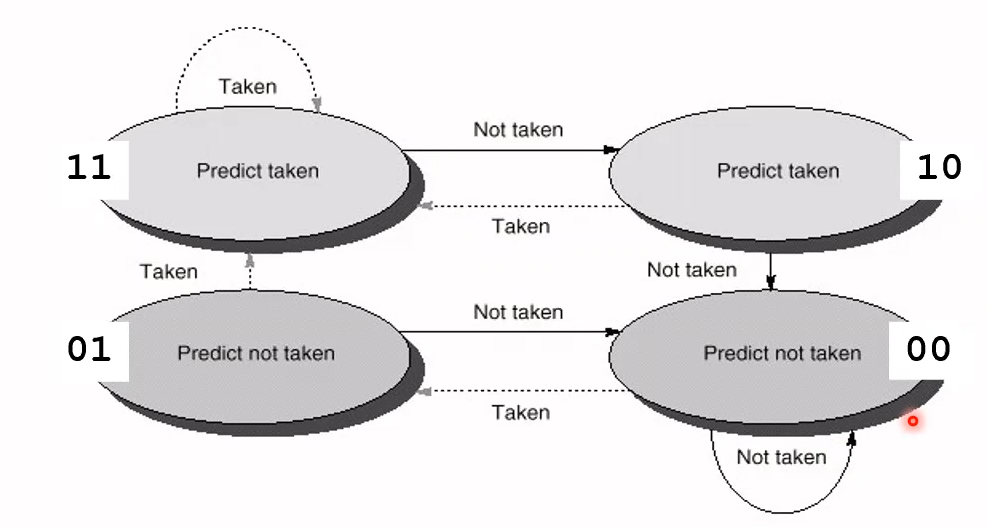
\includegraphics[width=0.8\textwidth]{two-bits-prediction-scheme.png}
    \caption{Two Bits Prediction Scheme}
    \label{fig:two-bits-prediction-scheme}
\end{figure}
Questi tipi di predittori sono stati evoluti, usando dei contatori (\textbf{n-bit saturating counter}), quando un salto viene preso il contatore aumenta altrimenti diminuisce, se il bit pi\`u significativo \`e settato ad 1 allora il branch viene preso, questo tipo di contatore di saturazione \`e molto facile da implementare.

\subsection{Correlation Predictors}
Altri tipi di predittori sono i \textbf{(m, n) predictors}, che si basano sulle dipendenze tra i risultati degli ultimi branch. Gli m-salti precedenti. Usano il comportamento degli ultimi \emph{m-branch} per scegliere tra $2^m$ diversi branch predictors, ognuno dei quali \`e un \textbf{predittore (BHT) a \emph{n-bit}}. Lo schema \`e molto semplice:
\begin{itemize}
    \item la storia degli ultimi \emph{m-branch} \`e immagazzinanta in in un \textbf{m-bit shift register}, dove ogni bit indica se il branch \`e stato preso oppure no, lo shift register andr\`a a selezionare tra le $2^m$ colonne;
    \item dall'indirizzo se scegli la riga e si controlla il valore a n-bit, la predizione sugli n-bit avviene come in una BHT, quindi si va a considerare il bit pi\`u significativo;
\end{itemize}
\begin{figure}[H]
    \centering
    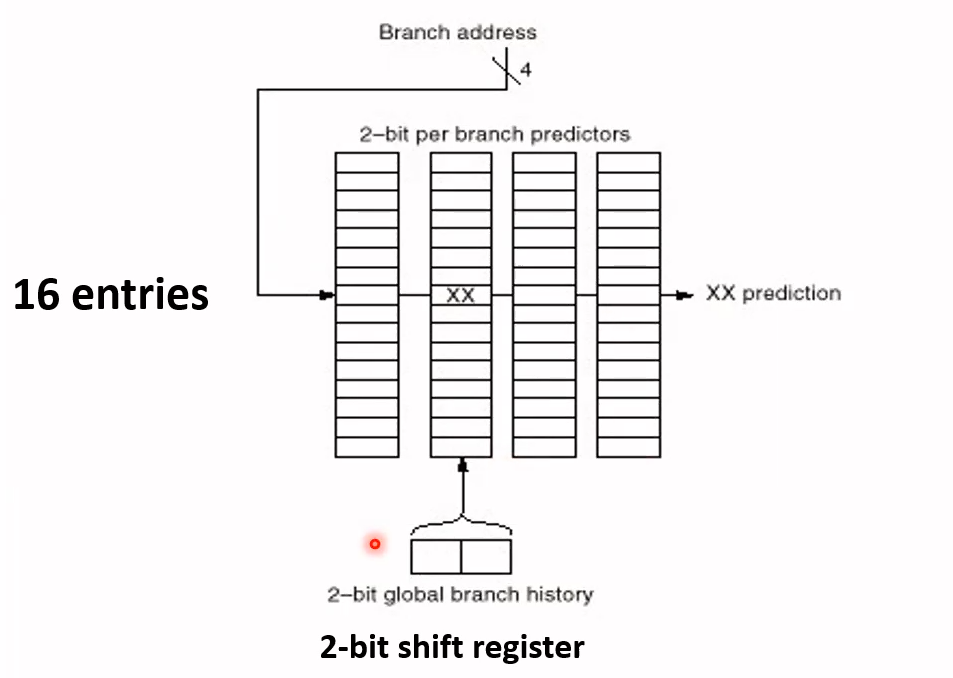
\includegraphics[width=0.8\textwidth]{predictor.png}
    \caption{(2,2) Predictor}
    \label{fig:predictor}
\end{figure}
Questi tipi di predittori non danno inforamazioni su dove saltare.

\subsection{Branch Target Buffer}
Il \textbf{Branch Target Buffer} viene usato nel MIPS, sfrutta delle memorie cache per funzionare. Ogni riga della del branch-target buffer contiene:
\begin{itemize}
    \item l'\textbf{indirizzo} del branch considerato;
    \item il valore \textbf{target} da essere caricato dentro il PC;
\end{itemize}
Con l'utilizzo del buffer il valore \`e caricato all'intero del PC alla fine della fase di IF, anche prima che l'istruzione di branch sia decodificata.
\begin{figure}[H]
    \centering
    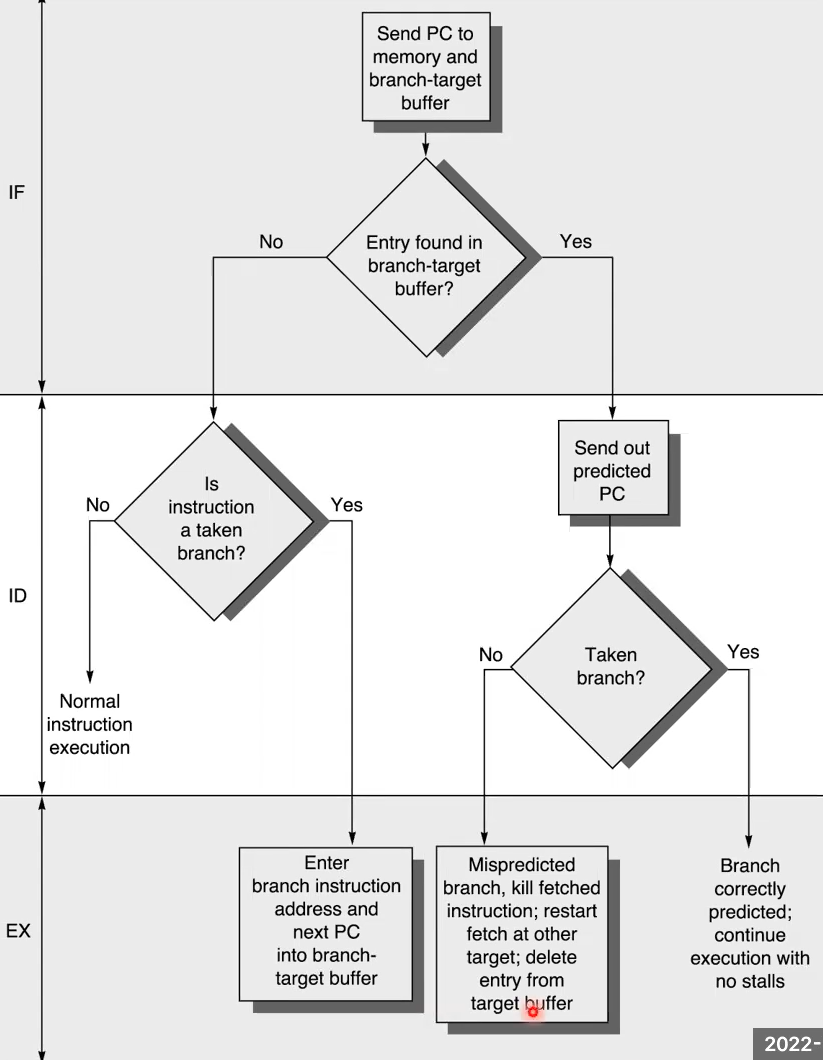
\includegraphics[width=0.7\textwidth]{comportamento-branch-target-buffer.png}
    \caption{Comportamento Branch Target Buffer}
    \label{fig:comportamento-branch-target-buffer}
\end{figure}
\begin{figure}[H]
    \centering
    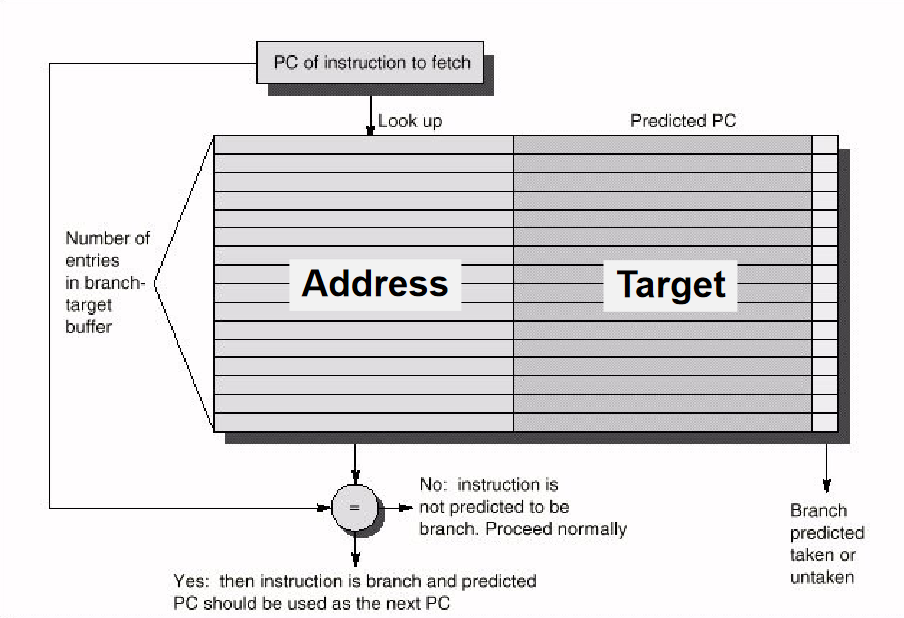
\includegraphics[width=0.8\textwidth]{architetture-branch-target-buffer.png}
    \caption{Architettura Branch Target Buffer}
    \label{fig:architetture-branch-target-buffer}
\end{figure}
Esistono anche due tipi di predittori chiamati \textbf{gselect} e \textbf{gshare}.



\newpage
\section{Schedulazione Dinamica}
La schedulazione dinamica si basa sul \textbf{riposizionamento in hardware} delle istruzioni per ridurre il numero di stalli causati dalla pipeline, pur mantenendo coerenza nei dati. Un modo per aumentare velocit\`a delle istuzioni e quella di permettere delle istruzioni \textit{out-of-order}, ovvero che delle istruzioni che vengono dopo possano terminare prima di quelle precedenti. Si ottiene questo grazie ad \textbf{unit\`a pipelined} e speciali buffer.
\begin{example}{}{}
    In questo l'istruzione \texttt{a} termina prima dell'istruzione \texttt{b}, b stalla a causo della dipendenza da f0, ma con istruzioni out-of-order a pu\`o essere eseguita mentre b sta stallando.
\begin{lstlisting}
c:  div.d f0, f1, f2
b:  add.d f1, f0, f0
a:  sub.d f3, f3, f3
\end{lstlisting}
\end{example}
Gli svantaggi di avere delle unit\`a separate sono:
\begin{itemize}
    \item WAR;
    \item WAW;
    \item eccezioni imprecise: prendendo l'esempio precedente, se sub.d finisce prima di div.d, e un eccezione  viene scatenata durante questa istruzione non possibile gestire le eccezioni in modo preciso, teoricamente sarebbe possibile ma ci sarebbe bisogno di un sacco di hardware costoso per poter immagazzinare lo stato del processore al momento dell'arrivo dell'eccezione;
\end{itemize}
Per fare questo l'ID deve essere diviso in due sezioni:
\begin{itemize}
    \item issue: decodifica dell'istruzione;
    \item read operands: vengono letti gli operandi e si controlla se non c'\`e nessun hazard, inoltre se un'unit\`a \`e piena l'istruzione viene stallata finech\`e non \`e possibile entrare;
\end{itemize}

\subsection{Algoritmo di Tomasulo}
L'\textbf{Algoritmo di Tomasulo} \`e un algoritmo hardware che rende possibile la schedulazione out-of-order e rende le singole unit\`a pi\`u efficenti. I punti chiave dell'algoritmo sono:
\begin{itemize}
    \item si traccia la validit\`a degli operandi;
    \item si introduce la possibilit\`a di rinominare i registri: ogni volta che viene fatto l'issue di un istruzioni i registri vengono rinominati con i registri di quella specifica reservation station, in questo modo si eliminano i WAW e RAW;
\end{itemize}
Sono molto importi le \textbf{reservation station}, il loro funzionamento \`e molto simile ad un buffer. Le fasi di un processore con l'algorimo sono:
\begin{itemize}
    \item IF: le istruzioni vengono immagazzinate in una coda FIFO;
    \item issue: viene prelevata la prossima istruzione dalla coda, se la matching reservation station \`e libera (no structural hazards), l'istruzione viene issued alla reservation station:
        \begin{itemize}
            \item con il valore degli operandi se in quel momento sono nei registri;
            \item altrimenti, con gli indentificatori delle reservation stations che produrranno l'operando;
        \end{itemize}
    \item execute: quando gli operandi sono disponibili (no RAW) e l'unit\`a \`e libera, viene eseguita altrimenti, viene monitorato il Common Data Bus;
    \item write result: il risultato viene scritto sul Common Data Bus a tutte le stazioni in attesa e nei registri, la reservation station viene segnata come libera;
\end{itemize}



\newpage
\section{Pipelining}
Esistono delle tecniche per portare le CPI sotto il numero 1, questo \`e possibile farlo attraverso il fetch di pi\`u istruzioni. Esistono due tipi di processori che possono farlo:
\begin{itemize}
    \item \textbf{superscalari}: hanno uno scheduling statico o dinamico;
    \item \textbf{very long instruction word (VLIW)};
\end{itemize}


\subsection{Static Scheduling}
Per implementare un processore superscalare viene creato un \textbf{issue packet}, dove viene fatto il fetch di due (o pi\`u) istruzioni contemporaneamente se in modo statico: una \`e load, store, branch o operazioni ALU e l'altra \`e una qualsiasi operazione FP, queste due istruzioni vengono chimate issue packet.
\begin{figure}[H]
    \centering
    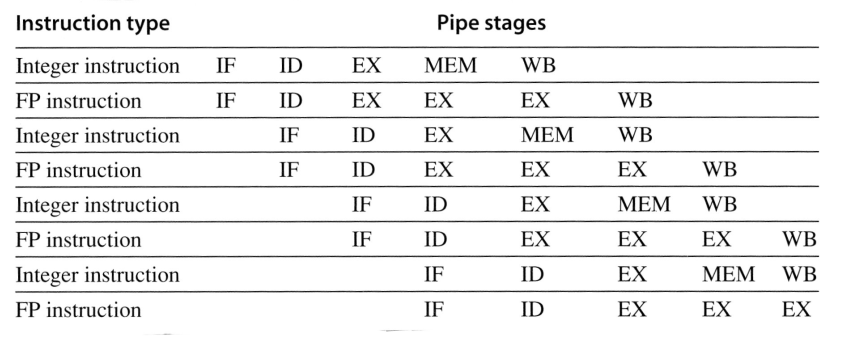
\includegraphics[width=0.8\textwidth]{issue-packet-example.png}
    \caption{Issue Packet Example}
    \label{fig:issue-packet-example}
\end{figure}
In un caso ideale si eseguiranno 0.5 istruzioni per colpo di clock. L'issue packet conterr\`a sempre una sola istruzione di branch. In questo caso l'unit\`a FP sar\`a pipelined o indipendente, in qualche modo \`e possibile ottere degli hazard, come: fare un un istruzione di load e subito dopo un'istruzione di write, oppure dei possibili RAW (read after write).

Nei sistemi moderni si utilizza una strategia statica in alcuni processori embedded con MIPS.


\subsection{Dynamic Scheduling}
Si pu\`o ottenere una schedulazione dinamica
Si ha un Common Data Bus (sistema di forwarding) comune, quindi viene duplicato. Suppoiamo di avere le seguenti istruzioni:
\begin{lstlisting}[language=]
loop:
    ls r2, 0(r1)
    daddiu r2, r2, 1
    sd r2, 0(r1)
    daddiu r1, r1, 4
    bne r2, r3, loop
\end{lstlisting}
Supponiamo che:
\begin{itemize}
    \item non ci sia speculazione:
    \begin{figure}[H]
        \centering
        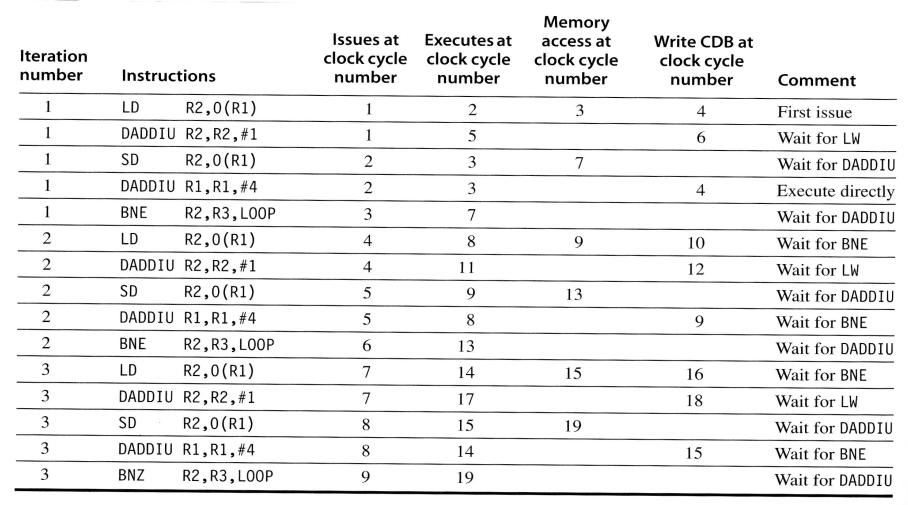
\includegraphics[width=0.8\textwidth]{dynamic-scheduling-senza-speculazione.png}
        \caption{Dynamic Scheduling Senza Speculazione}
        \label{fig:dynamic-scheduling-senza-speculazione}
    \end{figure}
    \item con speculazione:
        \begin{figure}[H]
            \centering
            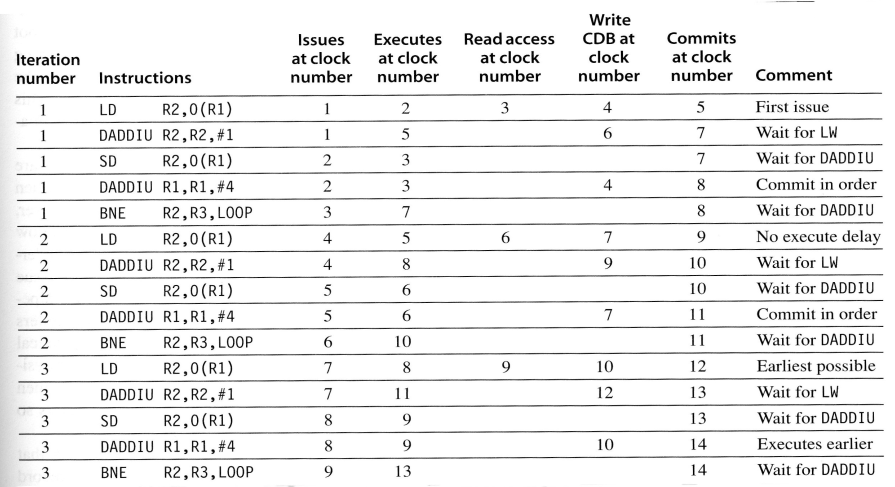
\includegraphics[width=0.8\textwidth]{dynamic-scheduling-con-speculazione.png}
            \caption{Dynamic Scheduling Con Speculazione}
            \label{fig:dynamic-scheduling-con-speculazione}
        \end{figure}
\end{itemize}



\newpage
\section{ARM}
Nei lab verr\`a usato il \textbf{Coretex M3} che fa parte di ARM9. ARM sviluppa architetture per tre categorie:
\begin{itemize}
    \item architetture embedded (SoC: system on a chip);
    \item sistem operativi;
    \item compilazione - supporto - debug tools
\end{itemize}


Uno dei moduli \`e il \textbf{Memory BIST}: questi parti del SoC servono per il collaudo del sistema, infatti duranta la pruduzione sul silicio le momoria potrebbere avere dei problemi fisici (quando si scrive in un registro il valore savato non \`e corretto o potrebbe intaccare quello dei registri vicini), infatti questi moduli non interagiscono direttamente con la logica del processore.

In un dispositivo ARM compliant la prima parte di codice che viene eseguita \`e il bootloader, per poi far partire il sistema operativo. Guadando la toochain, si parte dal codice assembly ARM, e dal codice C/C++, questi verranno compilati da un CROSS COMPILER, il risultato finala sar\`a un codice compilato con un ISA per ARM. Il risulatato sar\`a un eseguibile, con questo eseguibile sar\`a possibile usarlo in un simulatore di una scheda oppure caricarlo direttamente sulla scheda.


ARM cortex-M3 contiene 16 registri, tra cui il 15 \`e il PC. Il \textbf{barrel shifter} si avr\`a la possibilit\`a di creare valori immediati fino a 32 bit, sole se il valore contiene in qualche modo un replicazione all'interno di se stesso, inoltre ci permette di fare uno shift automatico del secondo registro su cui stiamo operando salvando un'istruzione.

Esistono alcuni casi particolari:
\begin{itemize}
    \item istruzioni \textbf{registro-registro}: dati i due registri Rn ed Rm, il primo entra direttamente nell'ALU, il secondo pu\`o essere modificato, al termine dell'operazione il risultato viene riportaro in un registro;
    \item ...
\end{itemize}


I vari moduli sono:
\begin{itemize}
    \item nested vectored interrupt controller;
    \item wake up interrupt controller interface: permette di mandare il dispositivo in sleep;
    \item memoria: interface code, memeory protection unit;
    \item SRAM e interfaccie periferiche: possibilit\`a di parlare con i timer;
    \item debug access port: permette di effettuare il debug anche attraverso il codice;
    \item ITM trace, ETM trace, data watchpoint, flash patch: moduli che permettono di fare il debug;
\end{itemize}

La pipeline \`e formata da:
...

Le istruzioni di branch comportano una perdita di due cicli. Quando si legge dalla memoria si perde un colpo di clock.

\subsection{Register}
Non tutti i registri sono general purpose, infatti:
\begin{itemize}
    \item 15: PC;
    \item 14: link register;
    \item 13: stack pointer: l'sp ha due versinoi;
\end{itemize}

L'instruction set utilizzato sar\`a il \textbf{thumb 2}, che prende le caratteristiche positive del thumb (a 16 bit) e dell'ARM, in thumb 2 esistono istruzioni a 16 e 32 bit, in questo modo i programmi sono pi\`u piccoli e le prestazioni sono simili all'ARM.

...

Ogni istruzione pu\`o essere eseguita in modo condizionato. L'architettura load e store si pu\`o utilizzare un formato di tre operandi.


\subsection{Instruction Set}
In questa architettura il PC \`e immagazzinato in r15, questo registro \`e modificabile, modificare il PC \`e importante quando ad esempio si ritorna da un subroutine, il registro r14 link register salva il valore di memoria di ritorno che andr\`a copiato nel PC. Il registro r13 \`e lo stack pointer, che permette di avere il valore dell'ultimo oggetto inserito, questo registro ha un valore iniziale, al termine del programma il valore dello stack pointer var\`a ricaricato con il suo valore iniziale che si trova all'interno della \textbf{interrupt vector table}, la posizione dello stack precedente si trova nell'index 0. Esiste anche il program status register \`e deviso in 3 registri, a seconda dell'operazione che si sta facendo si potrebbe accedere solo ad un parte del registro, vi sono dei flag delle operazioni aritmetiche, questo registro \`e diviso in:
\begin{itemize}
    \item application program status regiser (apsr);
    \item execution program status register (epsr);
    \item interrupt porgram status register (ipsr);
\end{itemize}

I flag sono:
\begin{itemize}
    \item Z zero;
    \item N negative;
    \item C carry;
    \item V overflow;
\end{itemize}

L'esecuzione condizionata delle istruzioni non vale solo per i salti, ma per ogni istruzione, nei 32 bit delle istruzioni ARM (comprese nella versione thumb 2), si hanno 4 bit che indicano il tipo di condizione che determina se l'istruzione viene eseguita oppure no, questo viene fatto leggendo i flag o secondo certe condizioni. Se si vuole che un istruzione modifichi un flag dobbiamo chiderlo esplicitamente, aggiungendo un \textbf{S} alla fine dell'istruzione.


v5.36 di Keil



Quando si organizza il codice si dovranno avere delle sezioni di codice. Nella memoria di codice readonly (quello che va in ROM) si possono definire delle costanti. Per salvare delle costanti in memoria esistono delle direttive per definire un tipo di dato (le direttive inziano con DC**).
\begin{lstlisting}[language=]
my_matrix   DCD  1, 2, 3, 4
            DCD  3, 4, 5, 6
            DCD  7, 8, 9, 1
            DCD  8, 9, 6, 3

my_const    DCD 10
\end{lstlisting}
Come ad esempio il salvataggio di una matrice e di una costante con dati.

Un'altra direttiva molto importante \`e quella di LTORG, ovvero dei \textbf{literal pool}, che permette al compilatore di accedere direttamente  ad alcune costanti che non sono accessibili direttamente, ad esmpio se un valore immediato \`e troppo grande (quando si fa un operazione come LDR r1, =0x12345678) viene salvato in questa zone dalla quale si pu\`o accedere.

Una volta fatte delle operazioni si possono valer salvare le variabili in memoria RAM, per fare questo si utilizza direttiva AREA, questa direttiva perende dei parametri:
\begin{itemize}
    \item |\emph{nome della sezione}|;
    \item \texttt{DATA / CODE}: definisce se la zona \`e e di codice o di dati;
    \item \texttt{READONLY / READWRITE}: definsce se si pu\`o leggere o scriver;
    \item \texttt{align=x}: definisce l'allineamento dei dati ...;
\end{itemize}

Per caricare un registro in memoria si utilizza un valore \textbf{pre-indicizzamento}: \texttt{load/store Rd, [Rt, <offset>]{!}}, se si usa ! il valore del registro viene incrementato prima di essere letto e quindi viene salvato se non si mette il ! il valore del registro viene incrementato dopo esser stato letto. L'offset pu\`o essere anche un valore salvato in un registro. Oppure usando si pu\`o usare un valore \textbf{pre-indicizzato}: \texttt{load/store Rd, [Rt], <offset>} 

La direttiva \textbf{EQU} ci permette di definire delle macro, avvero associare un valore ad un nome, esiste anceh la \textbf{RN} che chi permette di definire un alias per un registro.

Esempio di moltiplicazione di matrice, ogni elemento va moltiplicato per una costante e poi salvato:
\begin{lstlisting}[language=]
    AREA 	MY_DATA, DATA, READWRITE, align=3
NEW_MATRIX		SPACE 	5 * 4 * 4


    AREA    |.text|, CODE, READONLY


ROW 			EQU 	5
COL				EQU		4

ELEMENTS		EQU		ROW * COL

matrix 			RN		0
new_matrix		RN		1
i 				RN		2
j				RN		3
const			RN		4


; Reset Handler

Reset_Handler   PROC
    EXPORT  Reset_Handler             [WEAK]
        
    
    LDR matrix, =MATRIX
    LDR new_matrix, =NEW_MATRIX
    LDR	const, =CONSTANT
    LDR const, [const]
    MOV	i, #0
    MOV j, #0
    

ciclo_riga		MOV j, #0

ciclo_colonna	MOV	r6, #COL
    MUL r6, i, r6
    ADD r6, r6, j
    LDR r7, [matrix, r6, LSL #2]
    
    MUL r7, r7, const
    STR	r7, [new_matrix, r6, LSL #2]
    
    ADD j, j, #1
    CMP j, #COL
    BNE	ciclo_colonna
    
    ADD i, i, #1
    CMP i, #ROW
    BNE ciclo_riga      
    
    ENDP

MATRIX  		DCD  1, 2, 3, 4
    DCD  3, 4, 5, 6
    DCD  7, 8, 9, 1
    DCD  8, 9, 6, 3

CONSTANT    	DCD 10

    LTORG
\end{lstlisting}

\subsection{Stack}
Nel thumb2 lo stack \`e discendente, infatto quando si fa un push di un dato il valore dello stack decresce. Esistono anche gli stack ascendenti, entrambi si differenziano per essere full o empty,
che differenziano il modo in cui lo SP si muove.
\begin{figure}[H]
    \centering
    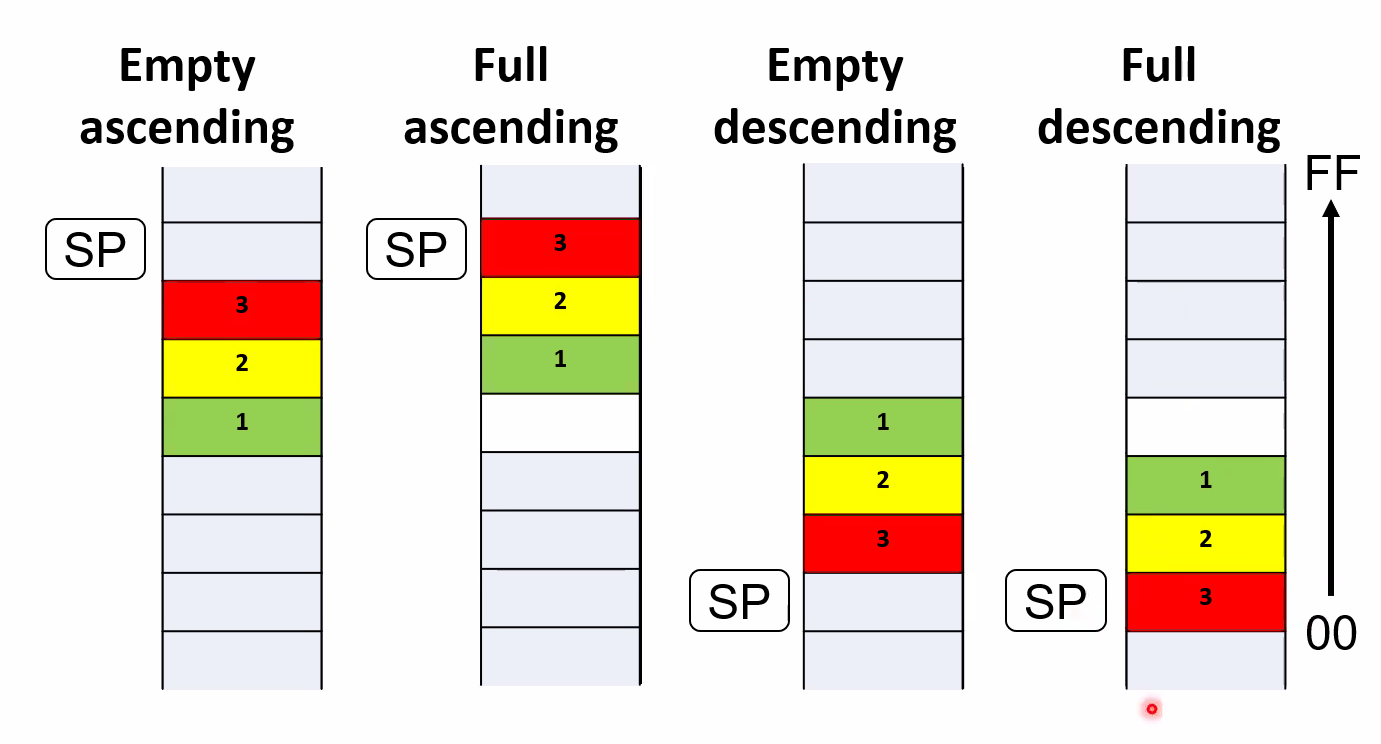
\includegraphics[width=0.8\textwidth]{tipi-di-stack.png}
    \caption{Tipi Di Stack}
    \label{fig:tipi-di-stack}
\end{figure}
Per iserire dei dati nello stack si utilizzano.
\begin{lstlisting}[language=]
LDM {xx} / STM {xx} <Rn>!, <regList>
\end{lstlisting}
Dovremmo fornire la lista dei registri, ad esempio \texttt{r0-r4, r10, LR}, il compilatore ordina tutto e poi vengono salvati. Il modo in cui avviene \`e salvano il registro pi\`u basso nella posizione pi\`u bassa dello stack. Lo SP non si pu\`o aggiungere nella lista, mentre il PC ed il LR sono mutuamente esclusivi.

I modi di indirizzamento sono IA (increment after, di default), DB (decrement before). Esistono delle istruzioni che implementano la PUSH e la POP nel caso di full descending o empy ascending. Nel nostro caso: \texttt{PUSH <regList> = STMDB SP!, <regList>; POP <regList> = LDMIA SP!, <regList>}.

Tutto questo serve per implementare delle \textbf{subroutine}, esistono delle istruzione che mi permettono di saltare e linkare (\texttt{BL <label>, BLX <Rn>}). Per determinare che un segmento di codice \`e una subroutine si utilizzano le keywork \texttt{PROC/FUNCTION, ENDP/ENDFUNC}. Esiste il problema del passaggio dei parametri, esistono 3 approcci:
\begin{itemize}
    \item dai registri;
    \item by reference;
    \item dallo stack;
\end{itemize}
Esistono comunque degli standard di chimata, il motivo \`e che potremmo chimare delle subroutine da codice C.

Esempi di codie che fa la sottrazione ed il valore assoluto passando i 3 tipi di argomenti:
\begin{lstlisting}[language=]
Reset_Handler 
    PROC

    ;registri
    mov r0, #42
    mov r1, #37

    BL sub1

    
    ;by reference
    mov r0, #42
    mov r1, #37
    LDR r3, =mySpace
    STAMIA r3, {r0, r1}
    BL sub2
    LDR r2, [r3]


    ;stack
    mov r0, #42
    mov r1, #37

    PUSH {r0, r1, r2} ;r2 = valore di ritorno
    BL sub3
    POP {r0, r1, r2}

    ENDP

sub1
    PROC
    PUSH {lr}

    CMP r0, r1
    SUBGE r2, r0, r1
    SUBLO r2, r1, r0

    POP {pc}

    ENDP

sub2
    PROC
    PUSH {r2, r4, r5, LR}
    LDMIA r3, {r4, r5}
    CMP r4, r5
    SUBHS r2, r4, r5
    SUBLO r2, r5, r4
    STR r2, [r3]

    POP {r2, r4, r5, PC}
    ENDP

sub 3
    PROC
    PUSH {r4, r5, r6, lr}
    LDR r4, [sp, #16]
    LDR r5, [sp, #20]

    CMP r4, r5
    SUBGE r6, r4, r5
    SUBLO r6, r5, r4

    STR r6, [sp, #24]

    POP {r4, r5, r6, pc}
    ENDP

\end{lstlisting}

\newpage
\section{Application Binary Interface}
Un ABI sono un insieme di standard per definire la comunzione tra due moduli di programmi binari, nel nostro caso quando in C deve essere chiamata un procedura assembler, vengono definiti come dovranno essere passati i parametri. L'interesse sar\`a relativo alla chiamate a procedure e alla gestione delle eccezioni. Un esmpio di ABI per i nomi dei registri:
\begin{figure}[H]
    \centering
    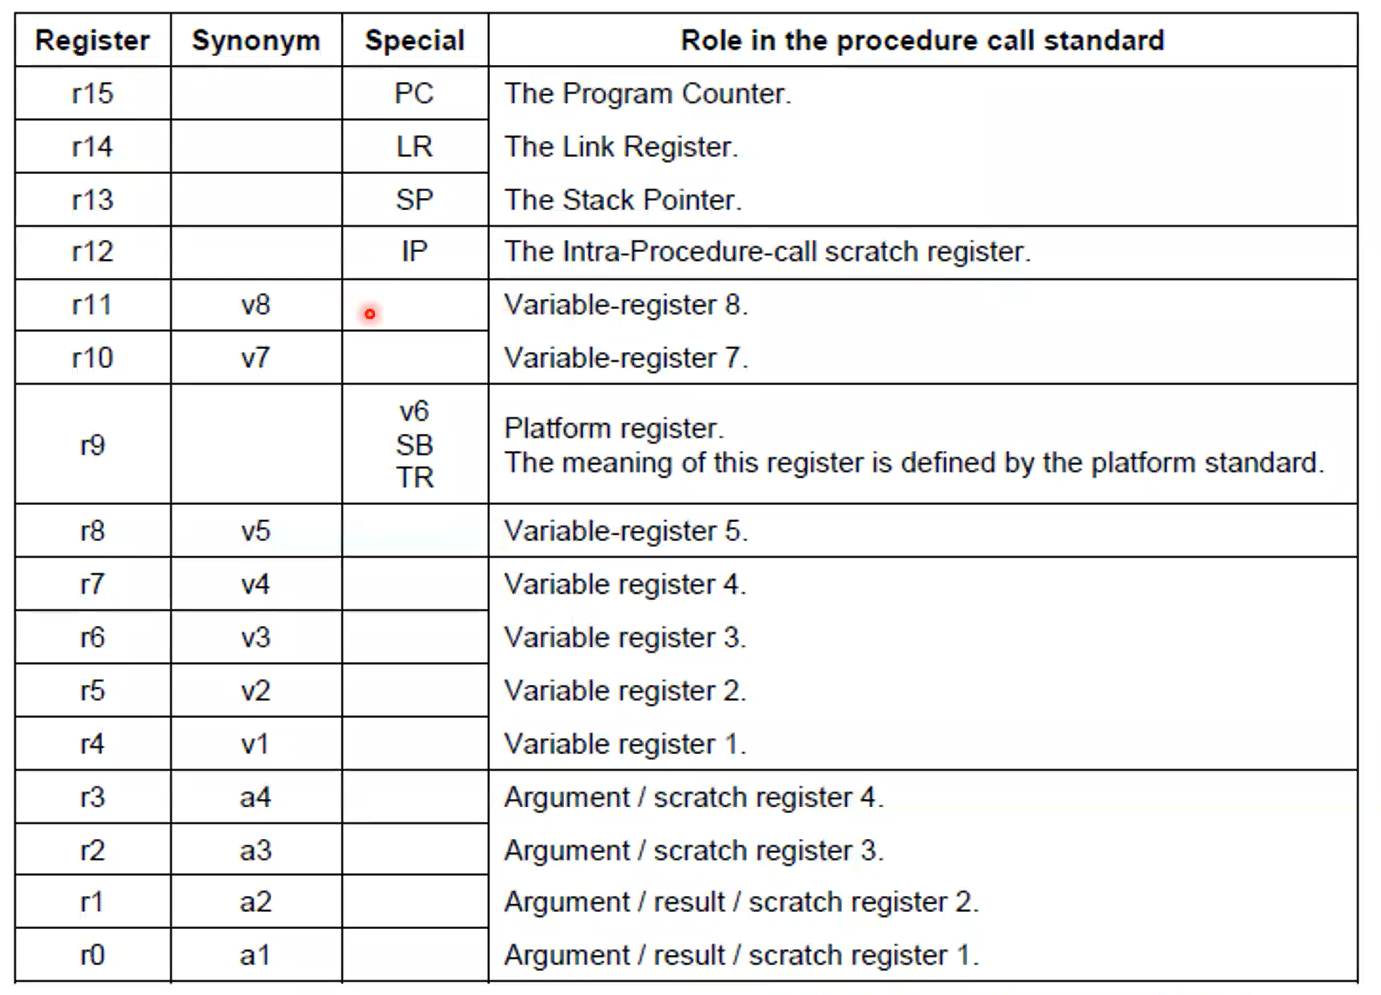
\includegraphics[width=0.8\textwidth]{register-abi.png}
    \caption{Register Abi}
    \label{fig:register-abi}
\end{figure}

\subsection{Supervisor Calls (SVC)}
Sono i Software Interrupt. Si dividono in Exception per le interruzoini sotfware e Interrupt che sono le interruzioni hardware. Nell'architettura ARM si possono per sollevare un interrupt si utilizza \textbf{SVC <id>}, dove l'id \`e l'indentificativo dell'interrupt.

La \textbf{Interrupt Vector Table} \`e una lista che specifica l'handler delle procedura che gestisce l'eccezione, fa eccezione solo la prima riga che \`e il valore iniziale dello stack pointer. Ogni riga ha uno spazio di 4 byte.
\begin{figure}[H]
    \centering
    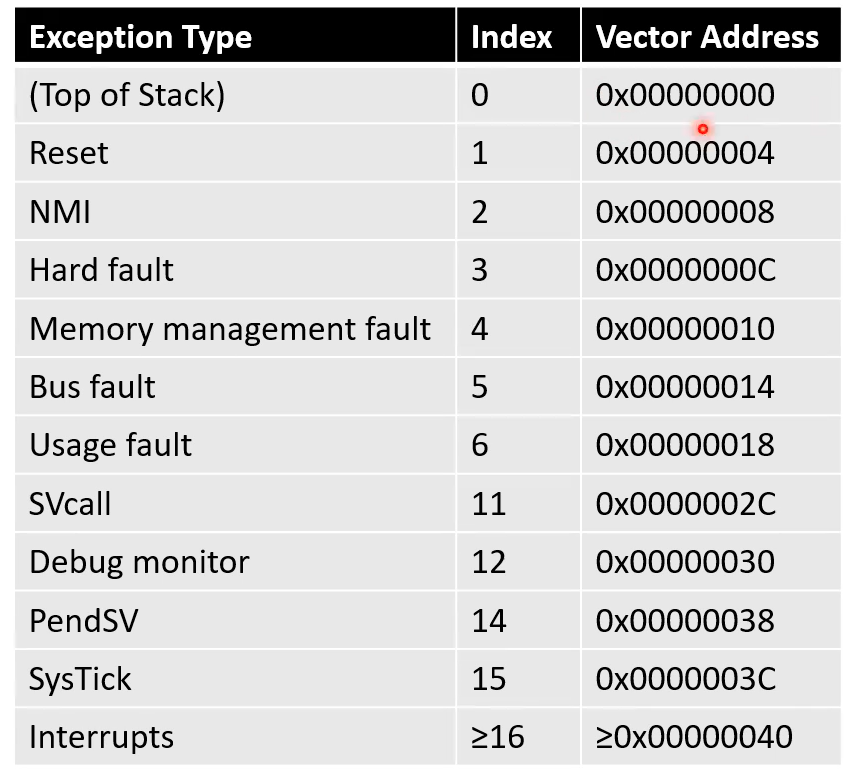
\includegraphics[width=0.8\textwidth]{ivt.png}
    \caption{Ivt}
    \label{fig:ivt}
\end{figure}
Ogni eccezione ha diverse priorit\`a, dopo l'hard fault \`e possibile programmarle. Le eccezioni hanno uno stato:
\begin{itemize}
    \item inattiva;
    \item attiva: un interruzione che sta venendo servita sul processore ma non \`e completata;
    \item pending: l'eccezione sta aspettando di essere schedulata sul processore;
\end{itemize}
Quando arriva un eccezione su un processore ARM, il processore deve saltare al suo handler, ma prima di fare ci\`o devono essere savati il registro dei flag, pc, lr, r12, r3-r0, questo processo viene fatto in automatico.

La sintassi delle svc \`e: \texttt{{label} SVC immediate}, il valore dell'immediato \`e a 8 bit, infatti l'SVC \`e una istruzione del thumb a 16 bit. Dopo l'esecuzione di una SVC, oltre ad i registri salvati nello stack, il LR viene caricato con un valore (diverso da quello di ritorno) detto \textbf{EXC\_RETURN}. 
\begin{figure}[H]
    \centering
    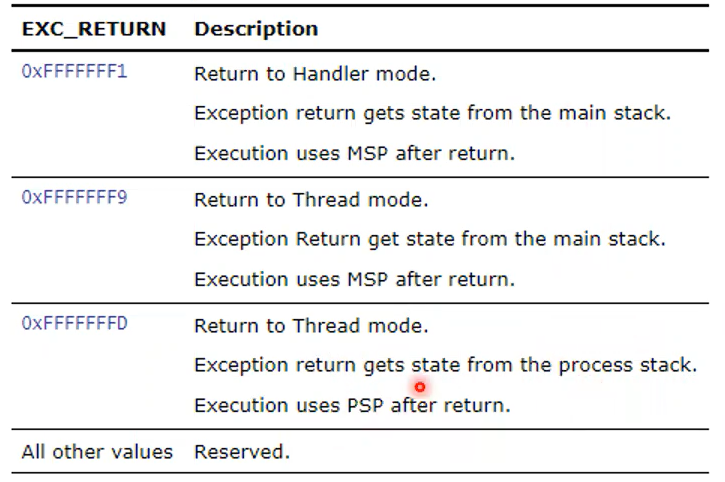
\includegraphics[width=0.8\textwidth]{exception-return.png}
    \caption{Exception Return}
    \label{fig:exception-return}
\end{figure}
Per leggere il valore dell'immediato si prende il valore del PC salvato nello stack, essendo che il valore viene compilato insieme all'istruzione, si pu\`o recuperare il valore leggendo l'istruzione precedente (perch\`e lo SP \`e incrementato) e facendo un BIC (bit clear) ed uno shift.

Si pu\`o utilizzare la MSR sono quando si \`e in handler mode, \texttt{MSR\{cond\} spec\_reg, Rn}.

Le modalit\`a di utilizzo sono:
\begin{itemize}
    \item \textbf{thread mode}: dopo un reset o dopo un'eccezione;
    \item \textbf{handler mode}: quando arriva un'eccezione;
\end{itemize}
I livelli di accesso sono:
\begin{itemize}
    \item \textbf{user level}: accesso limitato;
    \item \textbf{priviliged level}: accesso a tutte le risorse;
\end{itemize}
Handler mode \`e sempre a livello privilegiato.

A seconda del valore del registro di controllo si avr\`a lo PSP (process stack pointer) normale o un MSP (master stack pointer) quando ci si trova in handler mode. \`E importante ricordare che l'esecuzione \`e sempre in handeler mode quando viene chiamata un'eccezione, bisogna quindi definire delle sezioni di per lo stack, ovvero un sezione per il PSP ed un per il MSP.
\begin{lstlisting}[language=]
; stack segment
StackSize   EQU 0x00000200
            AREA STACK, NOINIT, READWRITE, ALIGN=3
            SPACE StackSize/2
StackProcess SPACE StackSize/2
__initial_sp
\end{lstlisting}
Qundo si vuole passare a thread mode ed impostare il valore del PSP, si deve:
\begin{lstlisting}[language=]
    MOV R0, #3  ; user mode
    MSR CONTROL, R0
    LDR SP, =StackProcess

    SVC 0x10
\end{lstlisting}
L'handler andr\`a gestito nel seguente modo:
\begin{lstlisting}[language=]
    PUSH {r0-r12, lr}
    
    TST lr, #2_1000
    MSREQ r1, PSP               ; thread mode
    LDREQ r0, [r1, #(14 + 6)*4]

    MSRNE r1, MSP               ; handler mode
    LDRNE r0, [r1, #(6)*4]

    BIC r0, 0xff000000
    LSR r0, #16
    
    ...

    POP {r0-r12, lr}
    BX lr
\end{lstlisting}



\section{ASM+C}
Per usare una funzione scritta in C da ASM si usa:
\begin{lstlisting}[language=]
Reset PROC
    EXPORT Reset
    IMPORT __main
    LDR r0, =__main
    BX r0
\end{lstlisting}

Per usare una funzione scritta in ASM da C si usa:
\begin{lstlisting}[language=C]
exter int ARM_funct(int, int, int);

int main(void)
{
    int i = 0xFF, j = 2, k = 3;
    volatile int r = 0;

    r = ASM_funct(i, j, k);
    return 0;
}
\end{lstlisting}
La funzione ASM\_funct \`e dischiarata come:
\begin{lstlisting}[language=]
    AREA asm_functions, CODE, READONLY
    EXPORT ASM_funct

ASM_funct
    ; save current SP for a faster access
    ; to parameters in the stack
    MOV r12, sp
    PUSH sp, {r4-r9,r10,r11,lr}

    LDR r4, [r12]
    LDR r5, [r12, #4]
    ; prepare return value
    MOV r0, r5

    PUSH sp, {r4-r9,r10,r11,lr}
    END
\end{lstlisting}

Se davanti ogni variabile non viene aggiunta la keyword \texttt{\textbf{volatile}}, il compilatore (in modalit\`a ottimizzata) potrebbe decidere di non usare un registro perch\`e pensa che sia inutile.




\section{Scheda}
\begin{figure}[H]
    \centering
    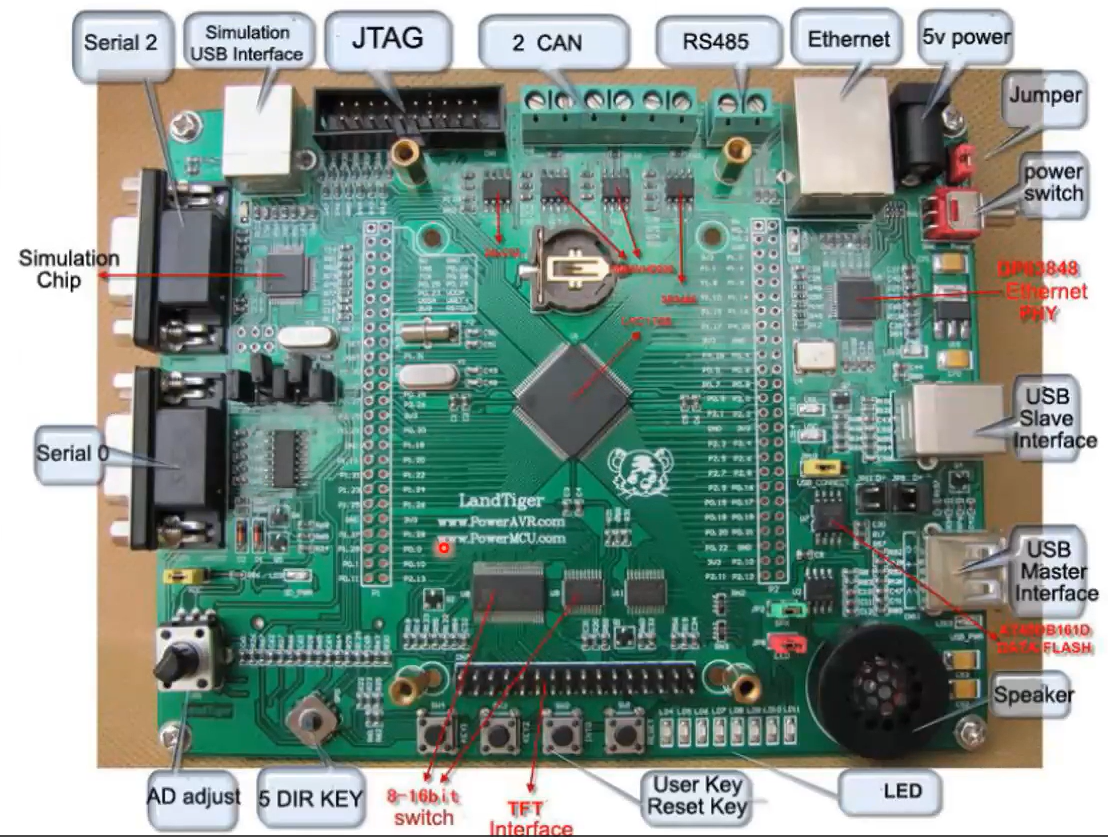
\includegraphics[width=0.8\textwidth]{landtiger.png}
    \caption{Landtiger}
    \label{fig:landtiger}
\end{figure}
Un struttura base di configurazione di una perfiriferica \`e:
\begin{lstlisting}[language=C]
PERIPHERA.h                 /* prototipi */
lib_PERIPHERA.c             /* funzioni base */
IRQ_PERIPHERA.c             /* interrupt service routine */
funct_PERIPHERA.c           /* funzioni avanzate */
\end{lstlisting}
Le i file da includere sempre sono:
\begin{lstlisting}[language=c]
system_LPC17xx.h
system_LPC17xx.c
core_cm3.c
\end{lstlisting}

Il file \texttt{lpc17xx.c} definisce delle costanti che corrispondono alle zone di memoria dei registri di sistema. Insieme vengono definite delle strutture per poter recuperare i dati presenti in quella zona di memoria.
\begin{figure}[H]
    \centering
    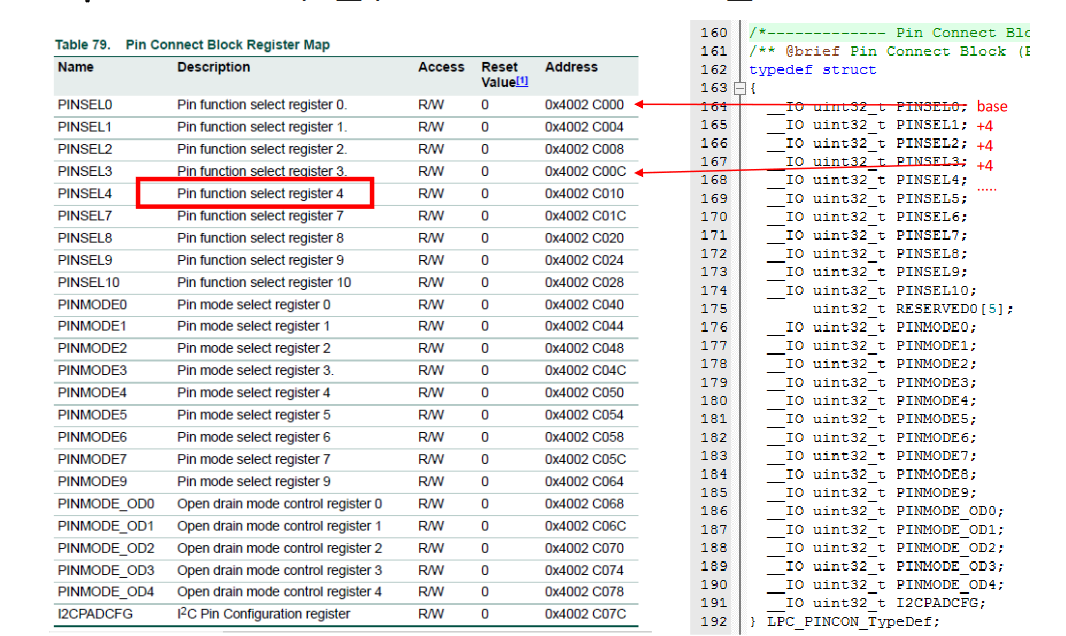
\includegraphics[width=0.8\textwidth]{pinsel-typedef.png}
    \caption{Pinsel Typedef}
    \label{fig:pinsel-typedef}
\end{figure}

\subsection{Interrupt}
Per configurare gli \textbf{switch} (bottoni) in modo far scatenare un eccezione si ha bisogno di di settare i bit della porta corripondente a 01, per abilitare l'eccezione EINT0, si fa:
\begin{lstlisting}[language=C]
void buttonInit(void) {
    //  Porta relativa all'abilatazione dell'eccezione dello switch 
    /* port P2.10 enabled with EINT */
    LPC_PINCON->PINSEL4     |= (1 << 20);
    // Registro gpio della direzione, definisce se la porta deve essere in input o in output
    /* port P2.10 defined as input */
    LPC_GPIO2->FIODIR       &= ~(1 << 10);

    // ...

    // Interrupt sensitivo al fronte di salita
    LPC_SC->EXTMODE = 0x7;

    // Abilitazione della interruzioni e delle priorit\`a
    NVIC_EnableIRQ(EINT0_IRQn);
    NVIC_SetPriority(EINT2_IRNQn, 1);
    
    // ...
}
\end{lstlisting}
Un esempio di handler sar\`a:
\begin{lstlisting}[language=C]
void EINT0_IRQHandler (void)	  
{
  LED_On(0);
  /* clear pending interrupt         */
  LPC_SC->EXTINT &= (1 << 0);     
}
\end{lstlisting}


Gli eventi che si scatenano possono essere periodici o asincroni. I tipi di interruzione possono essere: 

Si possono gestire le interruzioni in modo:
\begin{itemize}
    \item \textbf{polling}: gestito dal software, ovvero si usa un ciclo infinito per controllare periodicamente se dei registri relativi alle periferiche vengono modificati, in caso di modifica vengono gestite di conseguenza;
    \item \textbf{interrupt}: si devono configurare i periferici in modo che quando avviene un cambiamento, viene scatenata un'interruzione, la risposta a questi eventi saranno gestite dalle loro priorit\`a, per gestirle si usa la Nested Interrupt Vector Table;
\end{itemize}
Quando si vuole configurare un sistema con le interruzioni vanno inizializzate diverse istruzioni, come la configuraione dei periferici o dei valori iniziali da assegnare a dei registri, decidere la priorit\`a ed i perferici che possono interrompere, in oltre va fatto un \textbf{aknowledge} che un interruzione \`e avvenuta, questo consiste nel scrivere un valore in un registro (EXTINT) per non far risultare pi\`u l'interruzione come pending.

L'\textbf{interrupt controller}, che si trova all'interno del microcontrollore (solitamente), gestisce i piedini delle interruzioni e decide le priorit\`a dei vari tipi. Il cortex pu\`o gestire fino a 35 possibili interrupt.

Regitri utili:
\begin{itemize}
    \item per sarpere se un interrupt \`e attivo esite:
\begin{lstlisting}[language=c]
NVIC->IABR[0]
\end{lstlisting}
    questo registro contiene il valore (attivo/non attivo) dei primi 32 interrupt;
    \begin{figure}[H]
        \centering
        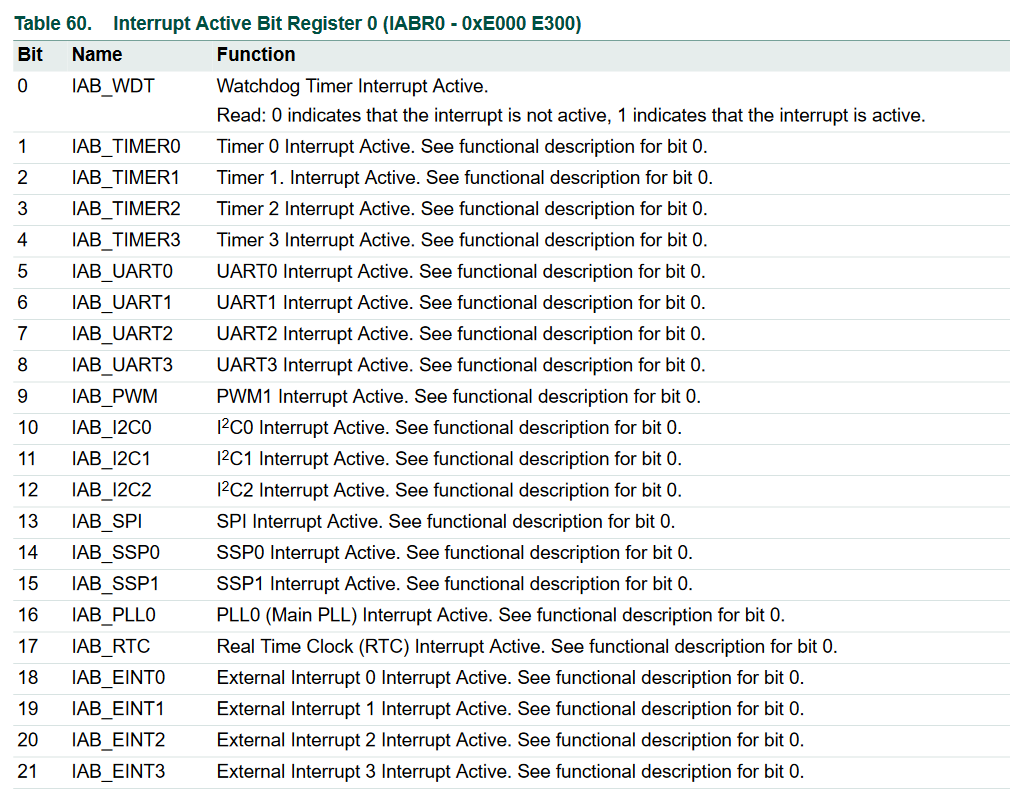
\includegraphics[width=0.8\textwidth]{iabr.png}
        \caption{Iabr}
        \label{fig:iabr}
    \end{figure}
    \item ...
\end{itemize}


\subsection{System Timing}
Alcuni sistemi (come il cortex), ci permette di utilizzare dei temporizzartori, o catturare l'intervallo di tempo tra due eventi.

Se si vuole che i timer contino per un certo periodo allora sfruttiamo la formula: $time[s] = count \cdot colckPeriod[s]$ (la costante che il simulatore vuole in input \`e il \emph{count}), ogni volta che passa questo periodo viene scatenata un eccezione.

I timer a disposizione nel sistema sono 4, 2 sono attivi di default metre gli atri 2 si possono accendere attraverso il PCONP. Per assegnare un timer count, si incorre nel problema che il valore potrebbe essere pi\`u grande della grandezza di un registro, per risolvere questo problema l'lpc1768 funziona con un \textbf{prescaler}, ovvero usa un valore a 64 bit che richiede due registri. I \textbf{match register} sono dei registri particolari che matchano il timer counter, ogni qual volta vengono matchati si possono fare varie operazioni, come lanciare un eccezione, modificare il valore dei match register o del timer, o controllare dei piedini.
\begin{figure}[H]
    \centering
    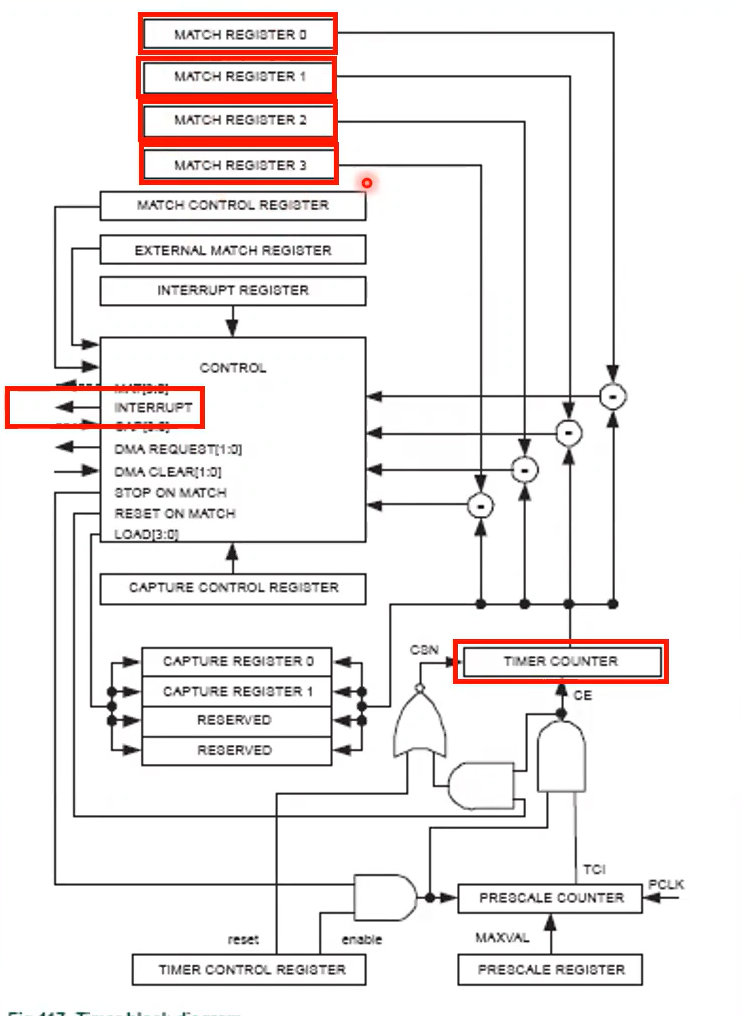
\includegraphics[width=0.8\textwidth]{match-registers.png}
    \caption{Match Registers}
    \label{fig:match-registers}
\end{figure}
La libreria dei match register ci facilita la configurazione attraverso il registro IRS, offrendo al match:
\begin{itemize}
    \item generazione di interrupt;
    \item reset il timer counter;
    \item stoppare il timer counter;
\end{itemize}
Ognuna di queste opzioni pu\`o essere abilitata o disabilitata attraverso i flag IRS che sono disponibili per ogni match register, infatti vengono detti match control register, visualizzabili nella seguente tabella.
\begin{figure}[H]
    \centering
    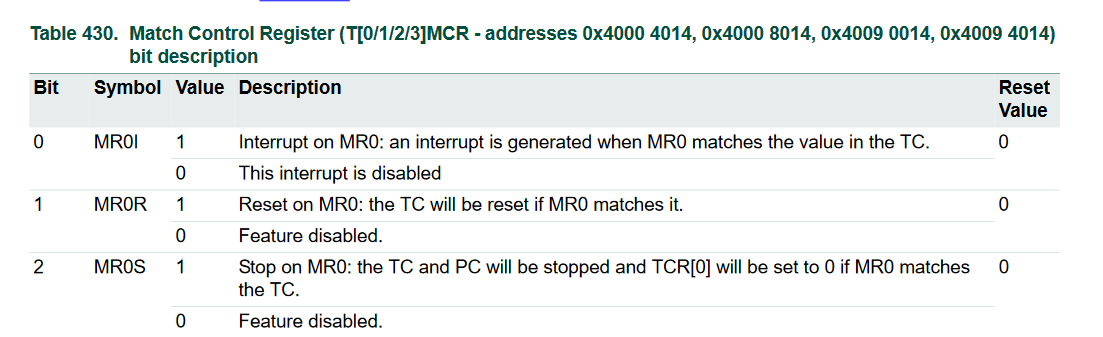
\includegraphics[width=0.8\textwidth]{irs-registers.png}
    \caption{IRS Registers}
    \label{fig:irs-registers}
\end{figure}


Si pu\`o anche utilizzare il \textbf{prescaler register}, che permette di utilizzare valori pi\`u alti per il match register, il prescaler funziona di divisore del clock, infatti utilizzandolo la nuova formula per il count \`e:
\[ count = time[s] \frac{frequency[1/s]}{(PR + 1)} \]
dove PR \`e il valore del prescaler.
\begin{figure}[H]
    \centering
    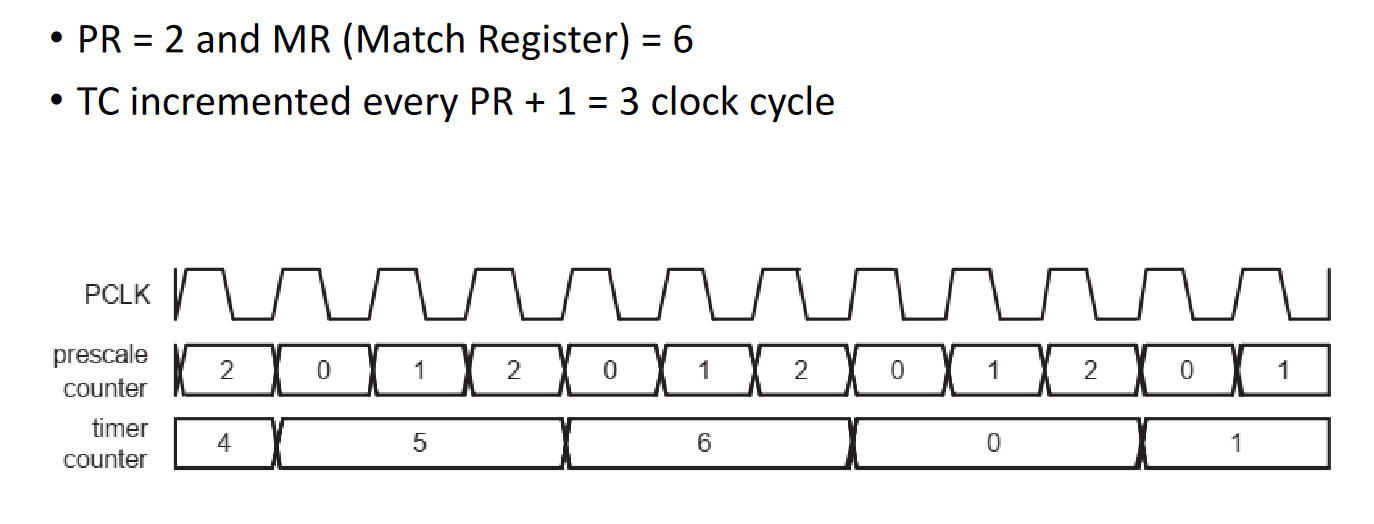
\includegraphics[width=0.8\textwidth]{prescaler.png}
    \caption{Prescaler}
    \label{fig:prescaler}
\end{figure}

Per inizializzare i timer:
\begin{lstlisting}[language=C]
int main()
{
    

}
\end{lstlisting}
\emph{La libreria dei timer (che fa un po schifo a detta del professore) possiede anche un wizard di configurazione}.


\subsection{Controllo del clock e della potenza}
Gli oscillatori esterni sono:
\begin{itemize}
    \item principale: pu\`o essere ad un cristallo esterno con frequenza tra 1MHz e 25MHz, attraverso una serie di processi aumenta la frequenza di base fino ad arrivare a 100MHz;
    \item interno ad RC (IRC): permette di far partire la scheda con un frequenza bassa, ha una frequenza di 4MHz, si pu\`o utilizzare per gestire il PLL;
    \item RTC: permette di fare misure temporali, arriva fino a 32kHz;
\end{itemize}
\begin{figure}[H]
    \centering
    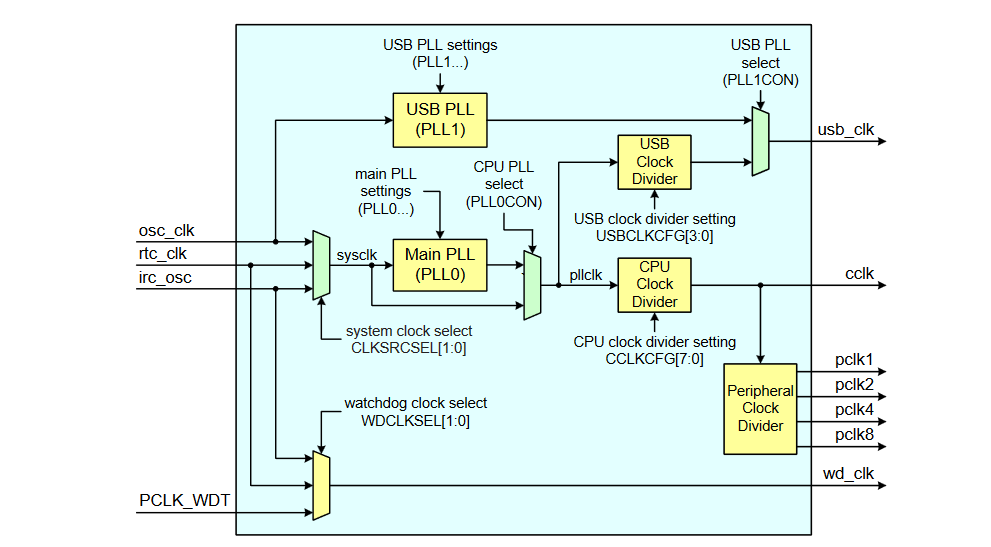
\includegraphics[width=0.8\textwidth]{clock-schema.png}
    \caption{Clock Schema}
    \label{fig:clock-schema}
\end{figure}
Fra i registri di configurazione esiste anche la scelta del clock, il registro si chiama \texttt{CLKSRCSEL}.
\begin{figure}[H]
    \centering
    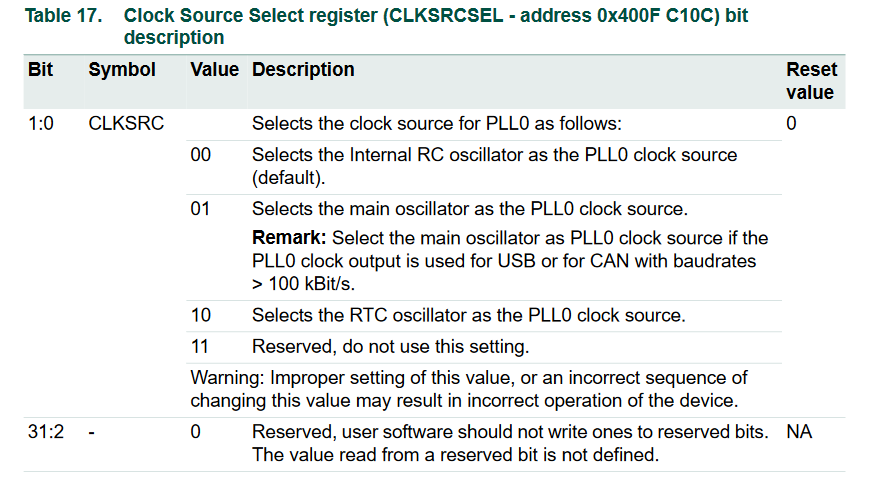
\includegraphics[width=0.8\textwidth]{clksrc.png}
    \caption{Clksrc}
    \label{fig:clksrc}
\end{figure}


Il controllo sulla potenza ci da delle modalit\`a diverse di consumo, i tipi di potenza possono essere:
\begin{itemize}
    \item sleep mode;
    \item deep sleep;
    \item power-down;
    \item deep power-down;
\end{itemize}
\emph{Le deep vanno evitate come la peste}.

Per utilizzare delle modalit\`a di consumo minore sono dei registri di configurazione, come il PCON (Power CONtrol register) ed il PCONP (Power CONtrol for Peripherals). Per entrare in modalit\`a di riduzione di potenza si utilizzano le istruzioni assembly \texttt{wfi} (\textbf{Wait For Intrrupt}) e \texttt{wfe} (\textbf{Wait For Exception}).

PCON contiene il PM0 ed il PM1 che permette di configurare il sistema in power down mode. Il BODRPM permette di controllare in un piedino se l'alimentazione sta scendendo, il sistema pu\`o implementare un interruzione per capire quando il sistema sta perdendo potenza (solitamente il threshold \`e a 2.2V), il problema \`e che quando si utilizza il power down mode il BODRPM dovrebbe essere disabilitato, ma in questo modo non ci si rende conto se il sistema si sta spegnendo davvero, allora si tiene attivo lo stesso.
\begin{figure}[H]
    \centering
    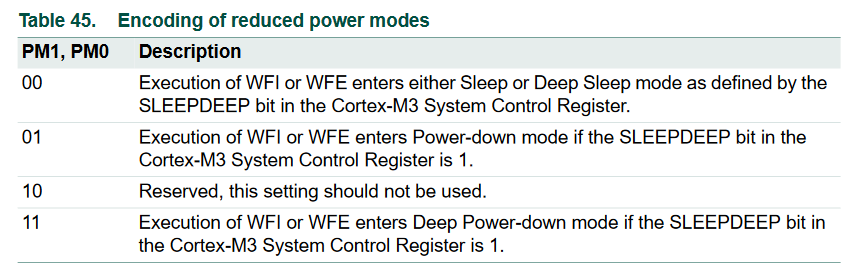
\includegraphics[width=0.8\textwidth]{power-modes.png}
    \caption{Power Modes}
    \label{fig:power-modes}
\end{figure}
Il registro di configurazione del power PCONP, ci permette di accendere l'alimentazione dei periferici, \`e importante ricordarsi che \textbf{se una periferica \`e spenta non \`e possibile leggere o scrivere sui registri realtive ad essa}.



\subsection{Debuoncing}
\begin{figure}[H]
    \centering
    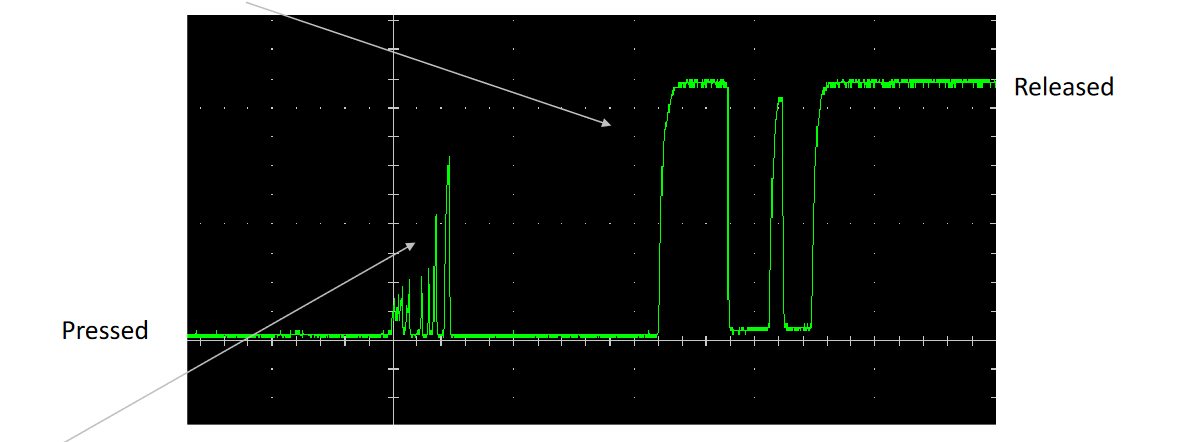
\includegraphics[width=0.8\textwidth]{bouncing-effect.png}
    \caption{Bouncing Effect}
    \label{fig:bouncing-effect}
\end{figure}
In molti casi quando si commuta un switch possono avvenire dei rimbalzi. Le soluzioni sono possono essere un'implementazione a livello hardware (costoso), oppure a livello software, ogni volta che arriva un interruzione da quel botton per un tot di secondi non si leggono pi\`u interruzioni da quel bottone, solitamente l'intervallo considerato \`e di 50ms.
\begin{figure}[H]
    \centering
    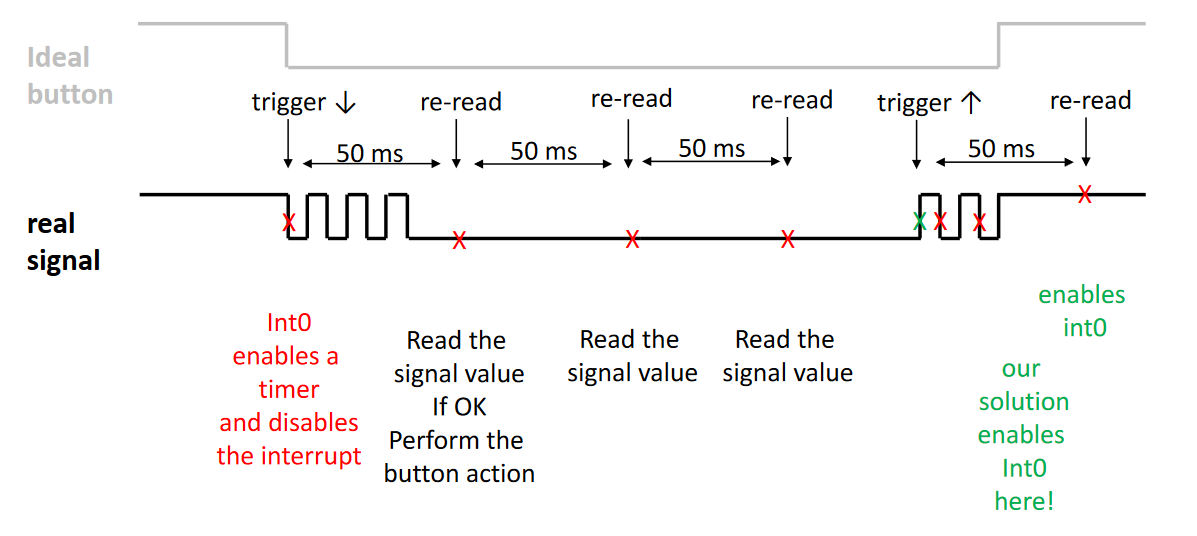
\includegraphics[width=0.8\textwidth]{debouncing.png}
    \caption{Debouncing}
    \label{fig:debouncing}
\end{figure}


\subsection{RIT}
Il RIT (Repetitive Interrupt Timer), \`e un timer di sistema che scatena delle eccezioni ad intervalli regolari, di default \`e spento infatti va abilitato
\begin{lstlisting}[language=C]
uint32_t init_RIT ( uint32_t RITInterval )
{
  LPC_SC->PCLKSEL1  &= ~(3<<26);
  LPC_SC->PCLKSEL1  |=  (1<<26);   // RIT Clock = CCLK
  LPC_SC->PCONP     |=  (1<<16);   // Enable power for RIT

  LPC_RIT->RICOMPVAL = RITInterval;      // Set match value
  LPC_RIT->RICTRL    = (1<<1) |    // Enable clear on match
					   (1<<2) ;	   // Enable timer for debug
  LPC_RIT->RICOUNTER = 0;          // Set count value to 0

  NVIC_EnableIRQ(RIT_IRQn);
  return (0);
}
\end{lstlisting}
Se si vuole gestire il debouncing dei pulsanti con il RIT, gestire pi\`u pulsanti per\`o \`e complicato.




\subsection{Schermo}
Lo schermo contiene due periferiche (gestite in modo separato) il touchscreen (capacitivo) e lo schermo (LCD).
\begin{figure}[H]
    \centering
    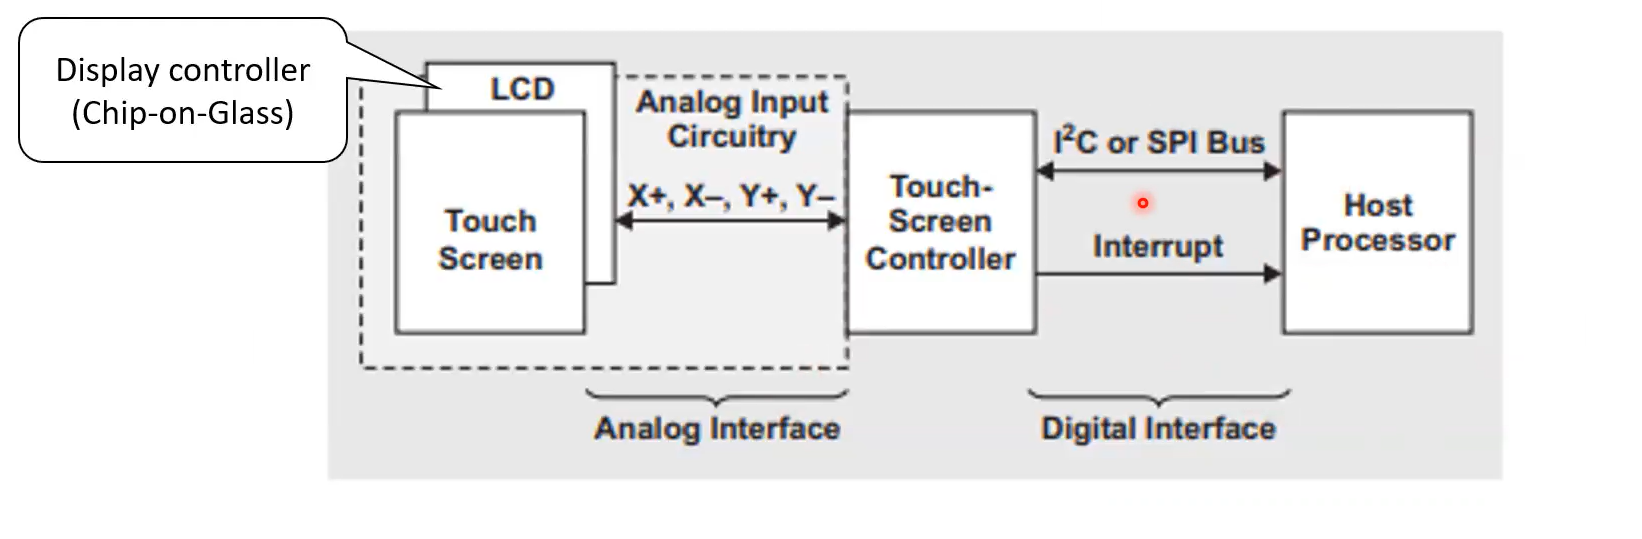
\includegraphics[width=0.8\textwidth]{schema-schermo.png}
    \caption{Schema Schermo}
    \label{fig:schema-schermo}
\end{figure}

Il contrllore del display fa avvenire parte delle sue comunicazioni in parallelo sulla porta 2, infatti quando si utilizza si potranno vedere i LED sfarfallare. Il controllore scrive sullo schermo una linea alla volta, lo schemro \`e 240RGBx320.


Per utilizzare lo schermo LCD si dovr\`a utilizzare la libreria. Quando si utilizza la libreria le operazioni di scrittura andranno a toccare dei registri di configurazione per scrivere il tipo di operazione da effettuare.

Mentre il touch \`e collegato ad un covertitore A/G che converte il tocco in due corrdinate.
\begin{figure}[H]
    \centering
    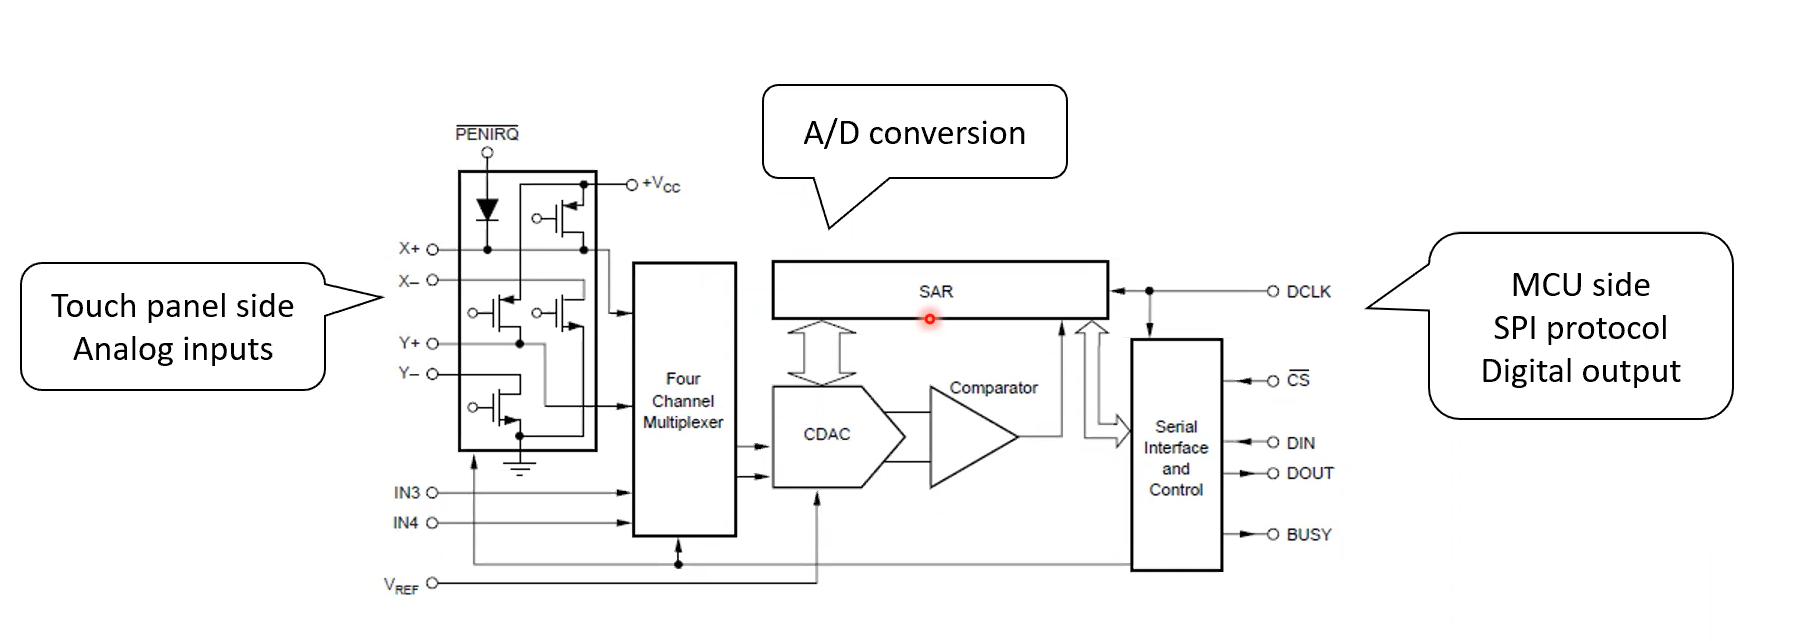
\includegraphics[width=0.8\textwidth]{convertitore-touch.png}
    \caption{Convertitore Touch}
    \label{fig:convertitore-touch}
\end{figure}
All'utilizzo del touch deve essere calibrato prima dell'utilizzo.
\begin{figure}[H]
    \centering
    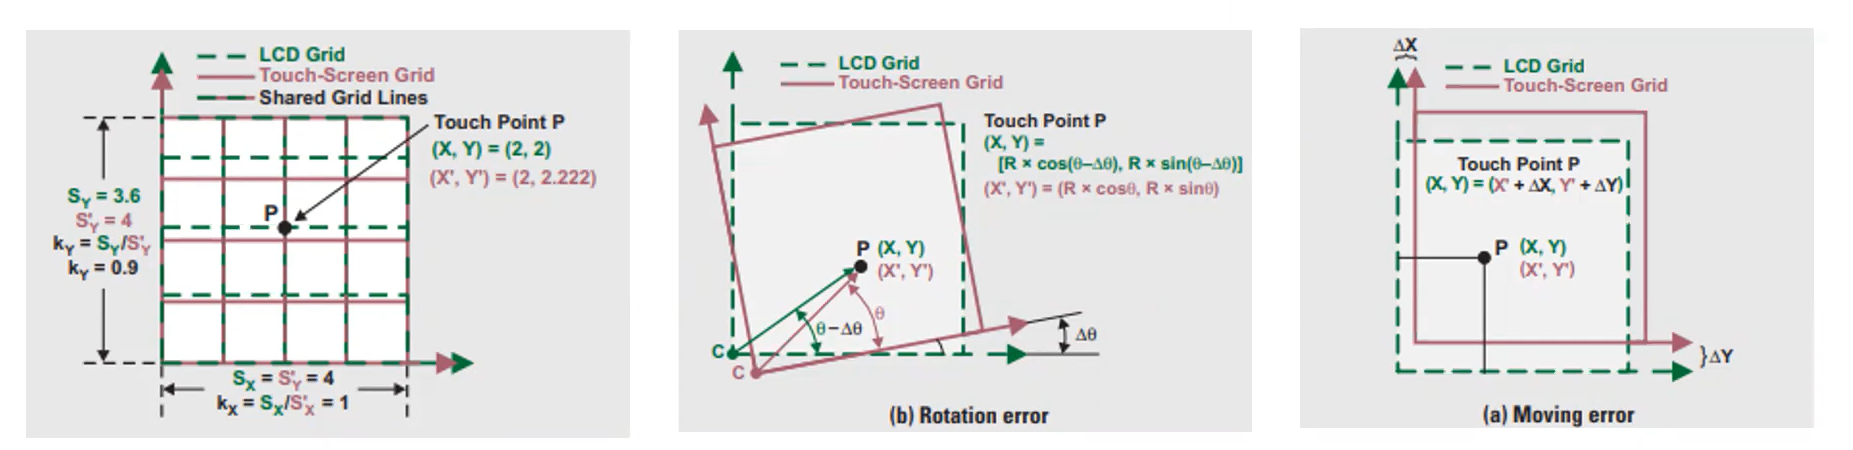
\includegraphics[width=0.8\textwidth]{errori-configurazione.png}
    \caption{Errori Configurazione}
    \label{fig:errori-configurazione}
\end{figure}



\newpage
\section{Analog Input and Output}
L'obbiettivo \`e quello di convertire degli segnali analogici in valori digitali, si ha bisogno di un ADC (Analog Digital Converter). La landtiger ha dei convertitori con frequenza di campionamento fino ai 13MHz. Gli ADC hanno anche risoluzione espressa in bit, questo in indica il range di intervalli omogenei in cui viene diviso il valore del segnale tra un minimo ed un massimo (quindi $2^{bit}$ valori totali possibili). L'ADC del landtiger ha:
\begin{itemize}
    \item \textbf{12 bit di precisione;}
    \item \textbf{8 input per il convertitore;}
    \item \textbf{13MHz di conversione massima;}
    \item \textbf{una conversione richiede 65 cicli};
    \item \textbf{range di volt tra 3V e 0V;}
    \item \textbf{pu\`o funzionare con power-down mode;}
    \item \textbf{la libreria di inizializzazione lo accende in automatico;}
\end{itemize}
Ogni ADDRx contiene l'ultimo valore campionato per ogni diverso convertitore.
\begin{figure}[H]
    \centering
    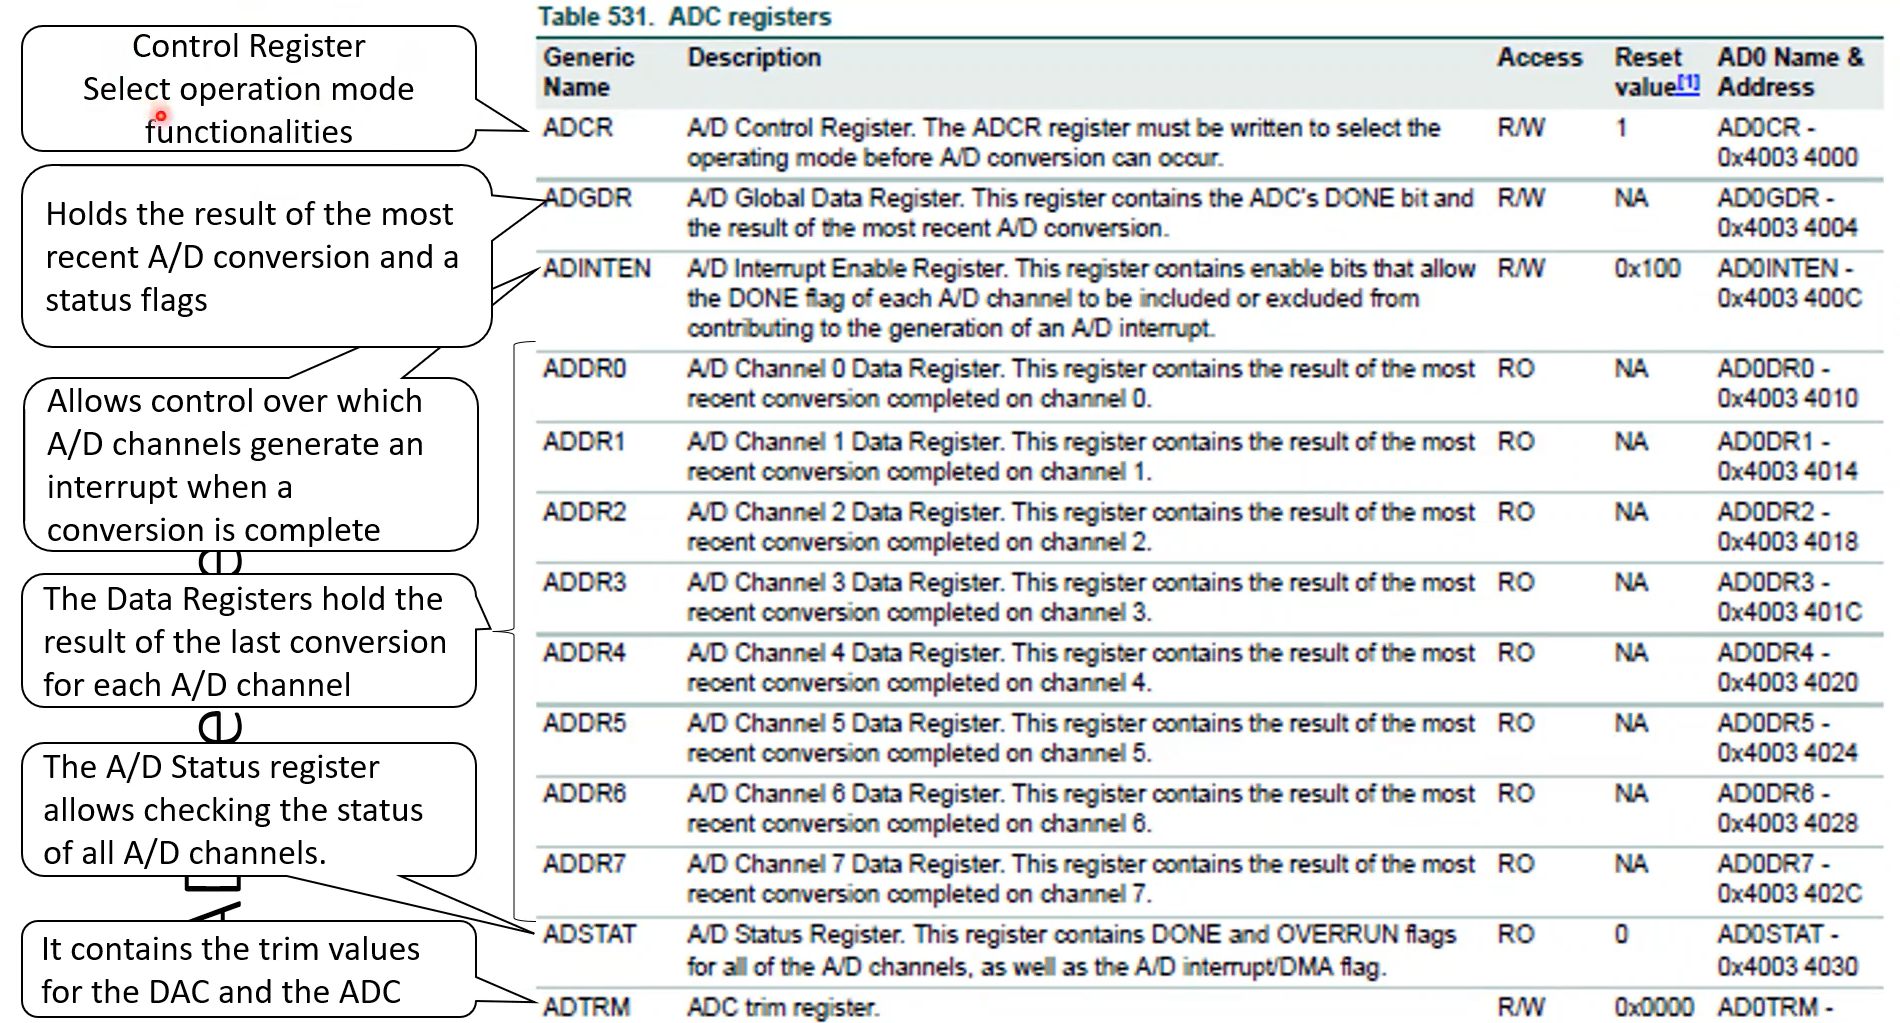
\includegraphics[width=1\textwidth]{registri-convertitore.png}
    \caption{Registri Convertitore}
    \label{fig:registri-convertitore}
\end{figure}
L'ADC ha come al solito una funzione di configurazione.
\begin{figure}[H]
    \centering
    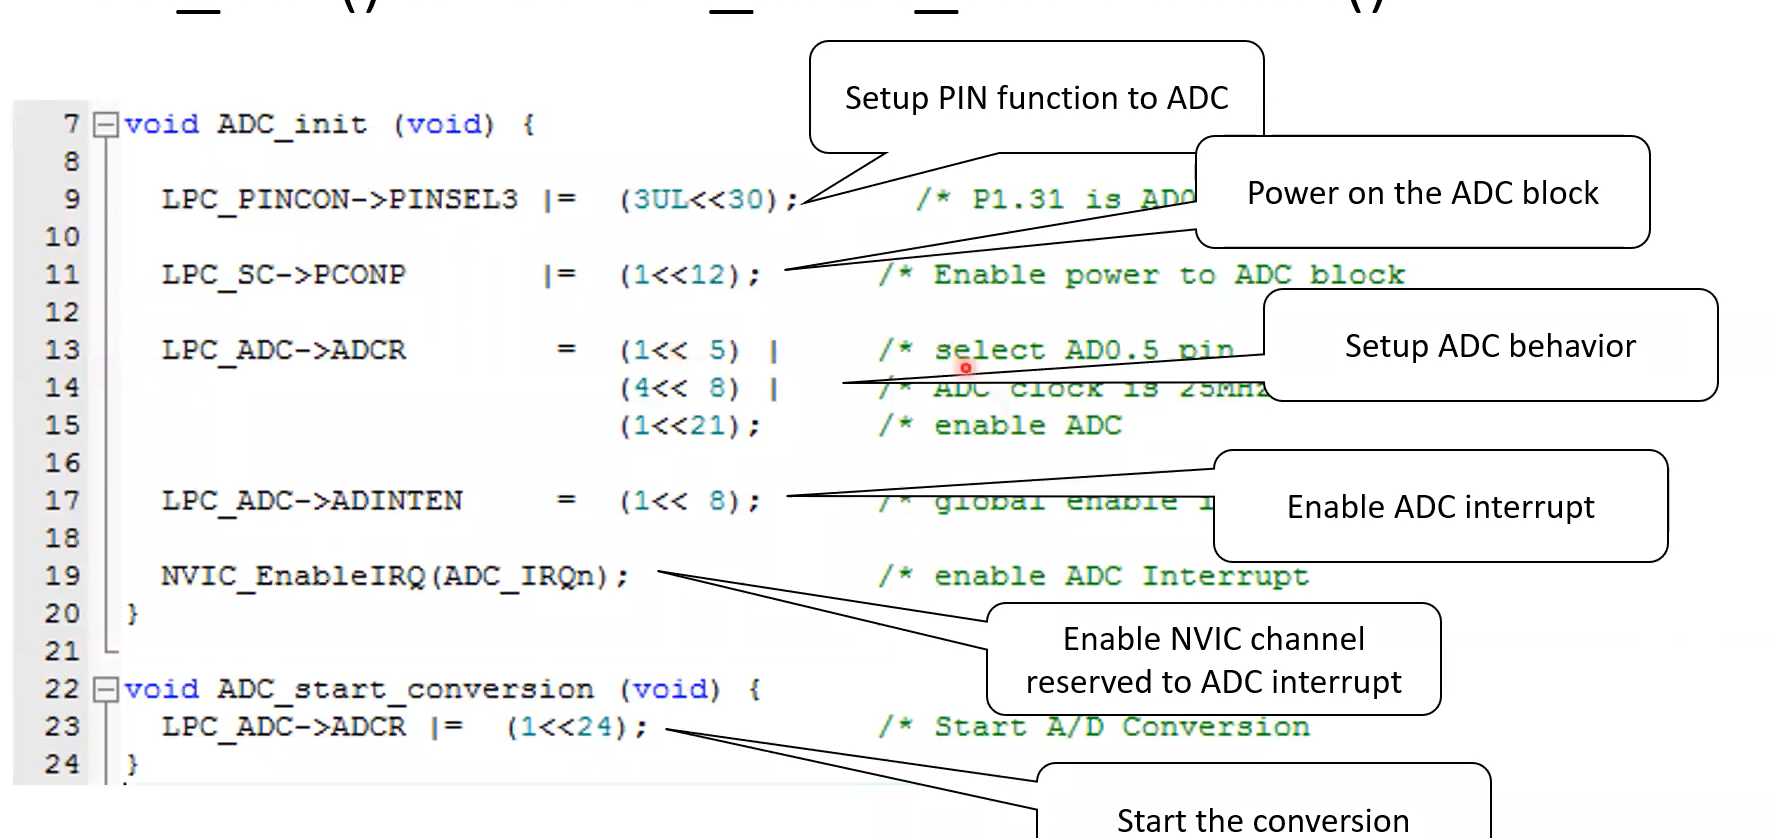
\includegraphics[width=0.8\textwidth]{adc-init.png}
    \caption{Adc Init}
    \label{fig:adc-init}
\end{figure}
Il convertitore ci permette anche di passare da digitale ad analogico, che \`e diverso da quello A/D:
\begin{itemize}
    \item \textbf{10 bit di precisione};
\end{itemize}
Nel caso della landtiger l'uscita analogica \`e collegata allo speaker.
\begin{figure}[H]
    \centering
    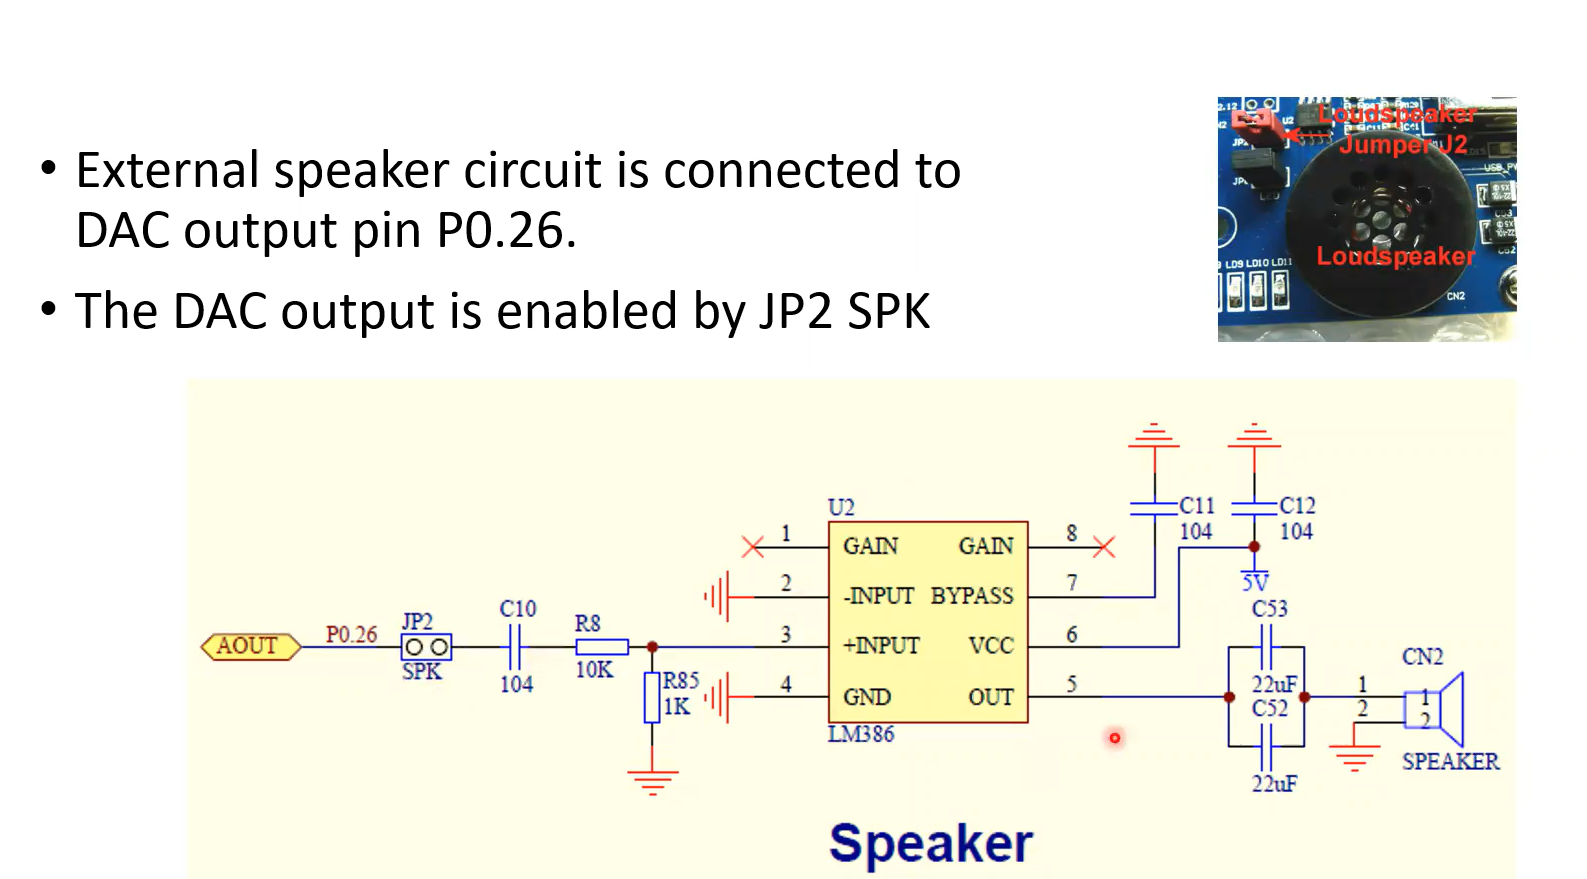
\includegraphics[width=0.8\textwidth]{uscita-speaker.png}
    \caption{Uscita Speaker}
    \label{fig:uscita-speaker}
\end{figure}
Possono essere ottenute delle note creando delle sinusoidi in uscita (magari anche sommate tra di loro). Si controlla l'uscita attraverso:
\begin{lstlisting}[language=c]
LPC_DAC->DACR = value << 6;
\end{lstlisting}
\textbf{si ricorda che \texttt{value} pu\`o essere solo di 10 bit}.
\begin{figure}
    \centering
    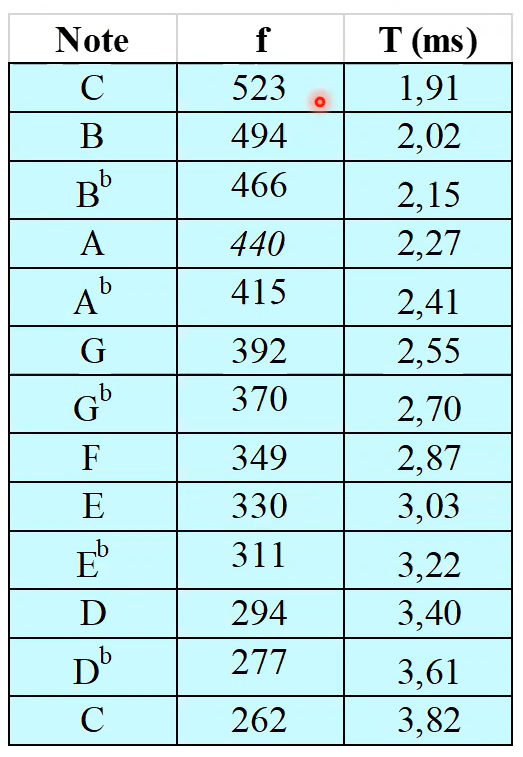
\includegraphics[width=0.4\textwidth]{note-speaker.png}
    \caption{Note Speaker}
    \label{fig:note-speaker}
\end{figure}





\newpage
\section{Esame}
Ricordarsi che l'ultima istruzione viene scartata, e quindi contata nel ciclo. Per fare il calcolo si fa: ...
\begin{figure}[H]
    \centering
    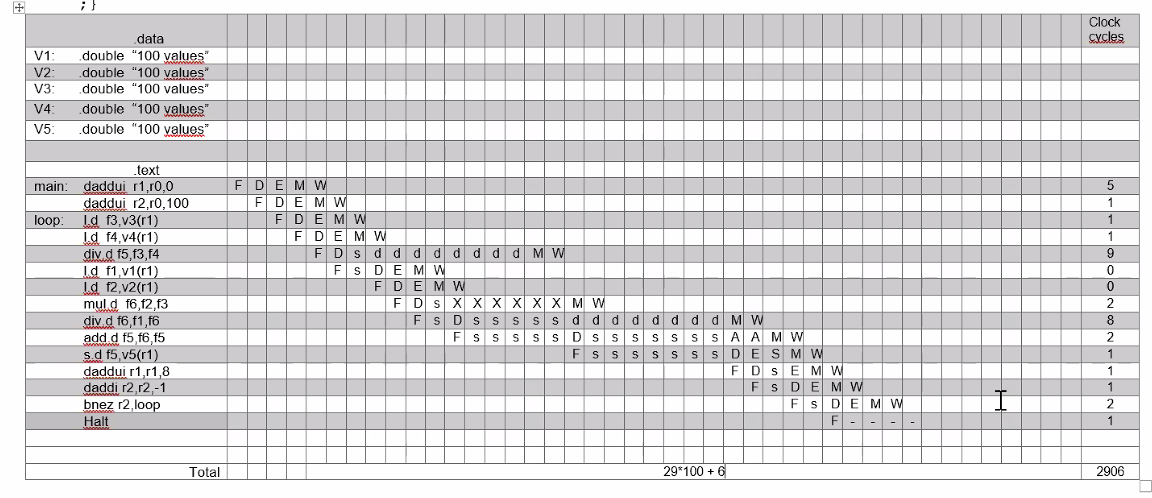
\includegraphics[width=0.8\textwidth]{esame-pipeline.png}
    \caption{Esame Pipeline}
    \label{fig:esame-pipeline}
\end{figure}








\end{document}
